\documentclass[12pt,a4paper]{article}

\usepackage[spanish,es-nodecimaldot]{babel}
\usepackage[utf8]{inputenc}
\usepackage[T1]{fontenc}
\usepackage{lmodern}
\usepackage{geometry}
\usepackage{booktabs}
\usepackage{longtable}
\usepackage{array}
\usepackage{amsmath}
\usepackage{graphicx}
\usepackage{float}
\usepackage{hyperref}
\usepackage{xurl}
\usepackage{enumitem}

\geometry{margin=2.5cm}
\hypersetup{colorlinks=true,urlcolor=blue,linkcolor=black}
\setlength{\emergencystretch}{3em}

\title{Construccion y especificaciones de la base trimestral \texttt{dt.csv}}
\author{Investigacion econometrica sobre Argentina}
\date{}

\begin{document}
\maketitle

\section{Objetivo y cobertura}

\texttt{dt.csv} es la base trimestral del analisis econometrico. Contiene 90 observaciones desde 2004-I hasta 2026-II. La base se construyo a partir de la
version actualizada de \texttt{datas.csv} y del ITCRM diario del Banco Central
de la Republica Argentina (BCRA). La columna temporal principal es
\texttt{fecha}, expresada en formato ISO y correspondiente al cierre de cada
trimestre: por ejemplo, \texttt{2004-03-31} representa 2004-I.

\section{Estructura temporal}

La base utiliza \texttt{fecha} como fecha de cierre trimestral y
\texttt{trimestre} como identificador numerico. La codificacion es:

\begin{center}
\begin{tabular}{cc}
\toprule
\textbf{Valor de \texttt{trimestre}} & \textbf{Trimestre}\\
\midrule
1 & I\\
2 & II\\
3 & III\\
4 & IV\\
\bottomrule
\end{tabular}
\end{center}

El formato ISO \texttt{AAAA-MM-DD} permite que Python y otros programas
reconozcan la variable directamente como fecha. En Python, la lectura
recomendada es:

\begin{verbatim}
import pandas as pd

df = pd.read_csv("dt.csv", thousands=",",
                 parse_dates=["fecha"])
df = df.sort_values("fecha").set_index("fecha")
df["periodo"] = df.index.to_period("Q")
\end{verbatim}

La variable \texttt{periodo} resultante toma valores como \texttt{2004Q1},
\texttt{2004Q2}, \texttt{2004Q3} y \texttt{2004Q4}. La codificacion romana
I--IV se reserva para la presentacion academica, mientras que los valores
numericos 1--4 se utilizan para el procesamiento.

\section{Fuentes y variables}

\small
\begin{longtable}{p{0.16\textwidth}p{0.27\textwidth}p{0.29\textwidth}p{0.20\textwidth}}
\caption{Definicion, fuente y transformacion de las variables}\\
\toprule
\textbf{Variable} & \textbf{Definicion} & \textbf{Fuente} & \textbf{Base o transformacion}\\
\midrule
\endfirsthead
\toprule
\textbf{Variable} & \textbf{Definicion} & \textbf{Fuente} & \textbf{Base o transformacion}\\
\midrule
\endhead
\texttt{pib} & PBI real de Argentina & INDEC, \url{https://www.indec.gob.ar/ftp/cuadros/economia/sh_oferta_demanda_desest_09_26.xls} & Serie desestacionalizada, en millones de pesos de 2004\\
\texttt{exportaciones} & Exportaciones de bienes & INDEC, \url{https://www.indec.gob.ar/indec/web/Nivel4-Tema-3-2-41} & Serie desestacionalizada, en millones de pesos de 2004\\
\texttt{importaciones} & Importaciones de bienes & INDEC, \url{https://www.indec.gob.ar/indec/web/Nivel4-Tema-3-2-41} & Serie desestacionalizada, en millones de pesos de 2004\\
\texttt{bc} & Saldo de bienes & Calculo propio & $BC_t=X_t-M_t$\\
\texttt{tc\_real} & Tipo de Cambio Real Multilateral & BCRA, \url{https://www.bcra.gob.ar/indices-de-tipo-de-cambio-multilateral/} & Base 17-12-2015=100; promedio diario trimestral\\
\texttt{covid} & Indicador de pandemia & Construccion propia & 1 en 2020-II--2020-III; 0 en otro caso\\
\bottomrule
\end{longtable}
\normalsize

\section{Construccion del ITCRM trimestral}

El ITCRM no es una cotizacion de pesos por dolar. Es un indice de
competitividad-precio multilateral. Su base es el 17 de diciembre de 2015,
igual a 100. La serie diaria se agrego mediante:

\[
ITCRM_t=\frac{1}{N_t}\sum_{d=1}^{N_t}ITCRM_{td},
\]

donde $N_t$ es el numero de observaciones disponibles en el trimestre $t$.
No se sustituyeron observaciones por cero ni se interpolaron manualmente.
El valor trimestral se incorporo en la columna \texttt{tc\_real}.

Como control de construccion, el promedio del ITCRM se obtuvo a partir de la
media de las observaciones diarias disponibles en cada trimestre.

\section{Construccion de la balanza comercial}

La balanza comercial se recalculo con las series de exportaciones e
importaciones:

\[
BC_t=X_t-M_t.
\]

El PBI, las exportaciones y las importaciones provienen de series
desestacionalizadas de oferta y demanda globales, expresadas en millones de
pesos a precios de 2004. Por tanto, el saldo comercial $BC_t$ conserva esa
misma unidad de medida.

Para 2004-I:

\[
BC_{2004-I}
=111457.782159446-76725.675769977
=34732.106389469.
\]

El resultado conserva todos los decimales disponibles en las series de origen.

\section{Variable retirada}

La columna \texttt{crisis\_eeuu} fue retirada de la base final porque no se
contaba con una fuente, fecha de inicio ni regla de construccion verificable
para la muestra. Esta decision mejora la reproducibilidad de la base.

\section{Uso econometrico}

El sistema principal puede incluir el PBI real, la balanza comercial y el
ITCRM:

\[
\{PBI_t,\ BC_t,\ ITCRM_t\}.
\]

La variable \texttt{itcrm\_bloo} debe utilizarse unicamente en un modelo
alternativo o prueba de robustez. No deben incluirse simultaneamente
\texttt{tc\_real} e \texttt{itcrm\_bloo}, puesto que son medidas alternativas de
la misma variable economica.

Antes de estimar un VAR o VECM deben realizarse pruebas de estacionariedad,
determinacion del orden de integracion, seleccion de rezagos, cointegracion y
diagnosticos de residuos.

\section{Metodologa y resultados del modelo}

Se siguio una secuencia de decisiones. Las pruebas previas no son modelos
adicionales: son controles que permiten definir la especificacion final y
comprobar si sus resultados son confiables.

\begin{enumerate}[leftmargin=*]
  \item Se construyo y ordeno la base trimestral, verificando fechas unicas,
  unidades y valores faltantes.
  \item Se definieron las variables del sistema: $\ln(PBI)$, $BC/PBI$ y
  $\ln(TC\ real)$. La razon $BC/PBI$ permite comparar el saldo comercial con el
  tamano de la economia.
  \item Se dividio la informacion antes de estimar. La muestra completa se
  uso para describir la historia y producir graficos. La muestra de
  entrenamiento se uso para todas las decisiones econometricas. La muestra
  reservada se uso unicamente para comparar pronosticos con datos observados.
  \item En el entrenamiento se aplicaron ADF, KPSS y Zivot--Andrews para
  estudiar estacionariedad, orden de integracion y una posible ruptura.
  \item Se escogio el numero de rezagos con AIC, BIC, HQIC y FPE.
  \item Se aplico Johansen para evaluar la relacion de largo plazo. Su
  resultado, junto con el orden de integracion, determino si correspondia VAR
  en niveles, VAR en diferencias o VECM.
  \item Se estimo el modelo seleccionado con COVID como variable exogena y se
  revisaron estabilidad, autocorrelacion, normalidad, causalidad de Granger,
  IRF, FEVD y CUSUM.
  \item Finalmente, se pronostico la muestra reservada y se calcularon RMSE,
  MAE y MAPE. Esta ultima etapa es la comprobacion fuera de muestra: esos
  datos no participaron en la seleccion del modelo.
\end{enumerate}

La muestra completa tiene 90 observaciones trimestrales, desde 2004-I hasta
2026-II. Para evaluar el pronostico se reservaron los ultimos ocho trimestres,
que corresponden a dos anos completos. Asi, el entrenamiento utiliza 82
observaciones, desde 2004-I hasta 2024-II, y la comprobacion fuera de muestra
abarca 2024-III--2026-II.

\begin{table}[H]
\centering
\caption{Uso de cada parte de la muestra}
\begin{tabular}{p{0.25\textwidth}p{0.25\textwidth}p{0.40\textwidth}}
\toprule
Parte & Periodo y observaciones & Uso \\
\midrule
Muestra completa & 2004-I--2026-II; 90 & Descripcion, graficos y construccion de la base. \\
Entrenamiento & 2004-I--2024-II; 82 & ADF, KPSS, Zivot--Andrews, rezagos, Johansen, estimacion y diagnosticos. \\
Comprobacion & 2024-III--2026-II; 8 & Pronostico fuera de muestra y comparacion con datos reales. \\
\bottomrule
\end{tabular}
\end{table}

Por tanto, los dos trimestres de 2026 si se incluyen en la base y se usan
para evaluar el pronostico, pero no se usan para elegir el rezago, calcular
Johansen ni estimar los coeficientes del modelo evaluado.

\begin{table}[H]
\centering
\caption{Estadisticas descriptivas de la muestra de entrenamiento}
\begin{tabular}{lrrrrr}
\toprule
Variable & N & Media & Desv. est. & Min. & Max. \\
\midrule
ln\_pib & 82 & 13.4017 & 0.1133 & 13.0613 & 13.5169 \\
bc\_pbi & 82 & -0.0193 & 0.0525 & -0.1194 & 0.0806 \\
ln\_tc\_real & 82 & 4.7678 & 0.2174 & 4.3684 & 5.1167 \\
\bottomrule
\end{tabular}
\end{table}


\subsection{Qué significan AIC, BIC, HQIC y FPE}

Estos indicadores ayudan a decidir cuántos trimestres anteriores debe usar el
modelo. No son cuatro modelos finales. Son reglas de comparacin: buscan
explicar bien los datos sin agregar rezagos innecesarios. Dentro de cada
criterio, el valor menor es preferible. En esta muestra todos eligieron un
rezago:

\begin{center}
\begin{tabular}{lc}
\toprule
Criterio & Rezago elegido \\
\midrule
AIC & 1 \\
BIC & 1 \\
HQIC & 1 \\
FPE & 1 \\
\bottomrule
\end{tabular}
\end{center}

\subsection{Las variables son integradas de orden uno}

El ADF busca evidencia de raíz unitaria y el KPSS busca evidencia de
estacionariedad. En niveles, para las tres variables se rechaza la
estacionariedad según KPSS y no se rechaza la raíz unitaria según ADF:
para $\ln(PBI)$ se obtuvieron $p_{\mathrm{ADF}}=0.0725$ y
$p_{\mathrm{KPSS}}=0.0100$; para $BC/PBI$, $0.3128$ y $0.0100$; y para
$\ln(TC\ real)$, $0.5190$ y $0.0100$, respectivamente. Por tanto, las
variables no son estacionarias en niveles.

En primeras diferencias, ADF rechaza la raíz unitaria y KPSS no rechaza la
estacionariedad en las tres variables. Los p-valores de ADF son inferiores a
0.001 y los de KPSS son 0.1000. En consecuencia, las tres variables se
clasifican como integradas de orden uno, $I(1)$. Los resultados completos
están en
\texttt{results/pruebas\_raiz\_unitaria.csv}.

\subsection{Qué mostró Johansen}

La prueba de Johansen verifica si las variables tienen una relación de largo
plazo. Para $r=0$, el estadístico de traza fue 49.5871, superior al valor
crítico de 29.7961 al 5\%, por lo que se rechazó la hipótesis nula. Para
$r=1$, el estadístico fue 10.8164, inferior a 15.4943, por lo que no se
rechazó la hipótesis nula. Para $r=2$, el estadístico fue 0.0166, inferior a
3.8415, y tampoco se rechazó la hipótesis nula.

El primer rango cuyo estadístico no supera el valor crítico es $r=1$.
Con tres variables, esto implica una relación de cointegración y justifica
la estimación de un VECM. El resultado completo se encuentra en
\texttt{results/cointegracion\_johansen.csv}.

\subsection{Modelo final}

Se estimó un VECM con las variables $\ln(PBI)$, $BC/PBI$ y
$\ln(TC\ real)$, incluyendo la dummy COVID como variable exgena. El modelo
usa un rezago del VAR en niveles, una relación de cointegración y cero
rezagos de las diferencias. La estimación se realiza con 82 observaciones.

\begin{table}[H]
\centering
\caption{Especificacin final de la estimacin}
\begin{tabular}{ll}
\toprule
Modelo & VECM \\
Variables endógenas & $\ln(PBI)$, $BC/PBI$, $\ln(TC\ real)$ \\
Variable exógena & Dummy COVID \\
Rezagos del VAR en niveles & $p=1$ \\
Rezagos de diferencias del VECM & $k_{\mathrm{ar\_diff}}=0$ \\
Rango de Johansen & $r=1$ \\
Muestra de entrenamiento & 2004-I--2024-II \\
Muestra de evaluación & 2024-III--2026-II \\
\bottomrule
\end{tabular}
\end{table}

La salida estadstica completa del modelo se encuentra en
\texttt{results/resumen\_modelo.tex}.

\begin{center}
\small
\begin{center}
\begin{tabular}{lcccccc}
\toprule
                & \textbf{coef} & \textbf{std err} & \textbf{z} & \textbf{P$> |$z$|$} & \textbf{[0.025} & \textbf{0.975]}  \\
\midrule
\textbf{const}  &       0.5441  &        0.561     &     0.970  &         0.332        &       -0.556    &        1.644     \\
\textbf{exog1}  &      -0.0304  &        0.021     &    -1.474  &         0.140        &       -0.071    &        0.010     \\
               & \textbf{coef} & \textbf{std err} & \textbf{z} & \textbf{P$> |$z$|$} & \textbf{[0.025} & \textbf{0.975]}  \\
\midrule
\textbf{const} &       1.6159  &        0.363     &     4.453  &         0.000        &        0.905    &        2.327     \\
\textbf{exog1} &       0.0036  &        0.013     &     0.267  &         0.790        &       -0.023    &        0.030     \\
               & \textbf{coef} & \textbf{std err} & \textbf{z} & \textbf{P$> |$z$|$} & \textbf{[0.025} & \textbf{0.975]}  \\
\midrule
\textbf{const} &       3.7387  &        1.176     &     3.180  &         0.001        &        1.435    &        6.043     \\
\textbf{exog1} &       0.0192  &        0.043     &     0.446  &         0.656        &       -0.065    &        0.104     \\
             & \textbf{coef} & \textbf{std err} & \textbf{z} & \textbf{P$> |$z$|$} & \textbf{[0.025} & \textbf{0.975]}  \\
\midrule
\textbf{ec1} &      -0.0451  &        0.047     &    -0.960  &         0.337        &       -0.137    &        0.047     \\
             & \textbf{coef} & \textbf{std err} & \textbf{z} & \textbf{P$> |$z$|$} & \textbf{[0.025} & \textbf{0.975]}  \\
\midrule
\textbf{ec1} &      -0.1354  &        0.030     &    -4.456  &         0.000        &       -0.195    &       -0.076     \\
             & \textbf{coef} & \textbf{std err} & \textbf{z} & \textbf{P$> |$z$|$} & \textbf{[0.025} & \textbf{0.975]}  \\
\midrule
\textbf{ec1} &      -0.3138  &        0.098     &    -3.186  &         0.001        &       -0.507    &       -0.121     \\
                & \textbf{coef} & \textbf{std err} & \textbf{z} & \textbf{P$> |$z$|$} & \textbf{[0.025} & \textbf{0.975]}  \\
\midrule
\textbf{beta.1} &       1.0000  &            0     &         0  &         0.000        &        1.000    &        1.000     \\
\textbf{beta.2} &       3.3005  &        0.444     &     7.434  &         0.000        &        2.430    &        4.171     \\
\textbf{beta.3} &      -0.2933  &        0.107     &    -2.730  &         0.006        &       -0.504    &       -0.083     \\
\bottomrule
\end{tabular}
%\caption{Det. terms outside the coint. relation & lagged endog. parameters for equation ln_pib}
\end{center}
\normalsize
\end{center}

\subsection{Interpretación sencilla}

El resultado debe leerse como un sistema de tres ecuaciones de corto plazo
con un término de corrección del error. El VECM combina los cambios
trimestrales de las variables con la relación de largo plazo estimada por
Johansen. No es una regresión donde un solo coeficiente explique todo el
efecto de la balanza sobre el PBI.

La relación de cointegración normalizada en $\ln(PBI)$ se aproxima a
\[
\ln(PBI)+3.3005\,BC/PBI-0.2933\,\ln(TC\ real)+\text{constante}=0.
\]
Sus coeficientes de largo plazo son estadísticamente significativos para
$BC/PBI$ ($p<0.001$) y $\ln(TC\ real)$ ($p=0.006$).

Los coeficientes de ajuste del término de error son $-0.0451$ para la
ecuación de $\ln(PBI)$ ($p=0.337$), $-0.1354$ para la ecuación de $BC/PBI$
($p<0.001$) y $-0.3138$ para la ecuación de $\ln(TC\ real)$ ($p=0.001$).
Por tanto, el ajuste hacia el equilibrio de largo plazo es estadísticamente
significativo en las dos últimas ecuaciones, pero no en la ecuación del PBI.

La salida de \texttt{fitted.summary()} también reporta los términos determinísticos
y la variable exógena en cada ecuación. En la ecuación de $\ln(PBI)$, la
constante es $0.5441$ ($p=0.332$) y el coeficiente de COVID es $-0.0304$
($p=0.140$); ninguno es estadísticamente significativo al 5\%. En la
ecuación de $BC/PBI$, la constante es $1.6159$ ($p<0.001$), mientras que
COVID presenta un coeficiente de $0.0036$ ($p=0.790$), sin evidencia de un
efecto estadísticamente significativo. En la ecuación de $\ln(TC\ real)$,
la constante es $3.7387$ ($p=0.001$) y el coeficiente de COVID es $0.0192$
($p=0.656$); únicamente la constante resulta significativa.

Debido a que $k_{\mathrm{ar\_diff}}=0$, el resumen no contiene coeficientes
de rezagos de las primeras diferencias. Por ello, la dinámica se interpreta
a partir del término de corrección del error, los términos determinísticos,
la variable COVID y la relación de largo plazo. La significancia de una
constante no debe interpretarse por sí sola como evidencia de causalidad
económica.

Esto no permite afirmar que la balanza comercial no tenga ningún efecto. Su
influencia puede aparecer mediante la relación de largo plazo, las dinámicas
de corto plazo y la reacción del sistema ante shocks. Por eso se revisan
también Granger, IRF y FEVD. La conclusión debe basarse en el conjunto de
resultados y no en un solo p-valor.

\subsection{Causalidad de Granger}

La prueba de Granger se interpreta como capacidad predictiva y no como
causalidad estructural definitiva. Para la hipótesis nula de que $BC/PBI$ no
causa a $\ln(PBI)$ se obtuvo un estadístico $F=0.591$ y un p-valor de
0.443. Por tanto, no se rechaza la hipótesis nula al 5\%: no se encuentra
evidencia de que la balanza comercial relativa mejore la predicción del PBI
en el sentido de Granger.

En sentido contrario, para la hipótesis nula de que $\ln(PBI)$ no causa a
$BC/PBI$ se obtuvo $F=6.460$ y un p-valor de 0.012. En este caso se rechaza
la hipótesis nula al 5\%, por lo que existe evidencia de capacidad predictiva
del PBI sobre la balanza comercial relativa. Estos resultados no contradicen
la existencia de una relación de largo plazo; describen únicamente la
dirección de la información predictiva de corto plazo evaluada.

\section{Rupturas, estabilidad y COVID}

Zivot--Andrews se utilizo como diagnostico de una ruptura endogena unica. Las
fechas sugeridas se ubican al comienzo de la muestra, por lo que no se
incorporaron automaticamente como dummies: podrian estar captando el inicio
del periodo observado. La pandemia se trata separadamente mediante la dummy
\texttt{covid}, definida con valor uno en 2020-II y 2020-III.

La prueba CUSUM no rechaza la estabilidad al 5\% en ninguna ecuacion:
los p-valores fueron 0.3185 para $\ln(PBI)$, 0.6545 para $BC/PBI$ y 0.9900
para $\ln(TC\ real)$. Estos resultados no prueban que no existieran shocks, sino
que no se detecta inestabilidad estadisticamente significativa en los residuos
del sistema estimado.

\begin{figure}[H]
\centering
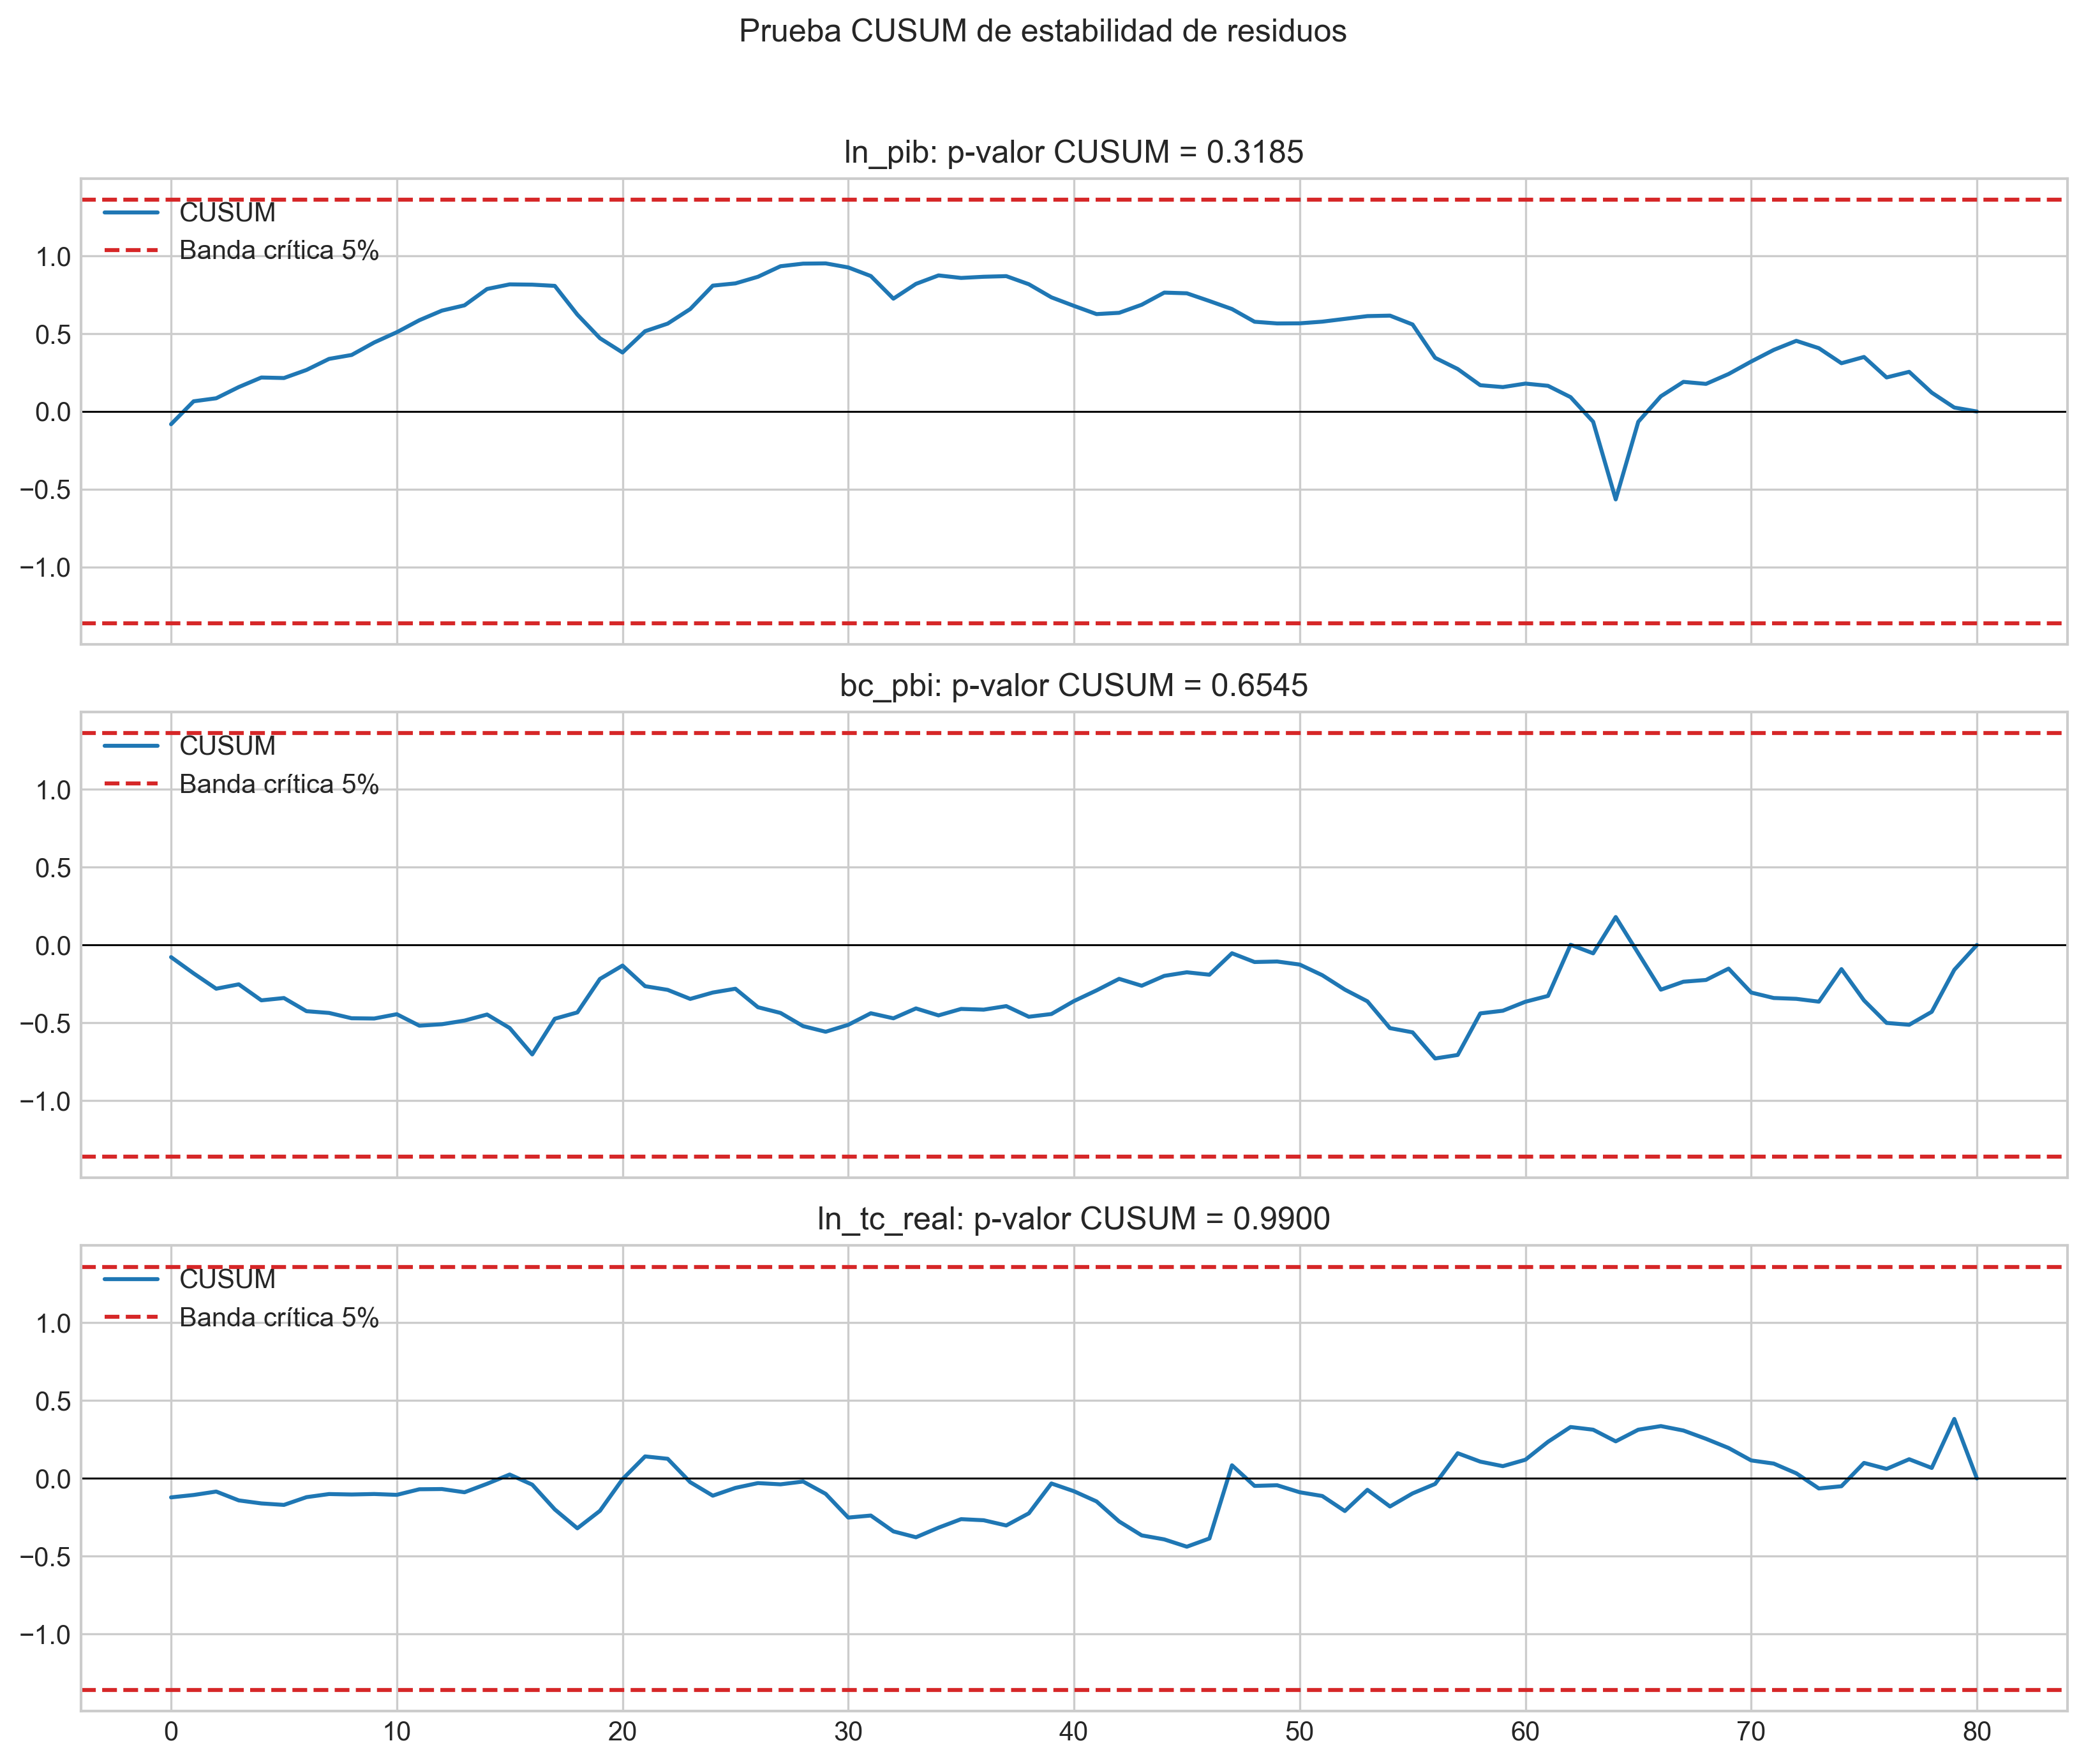
\includegraphics[width=0.92\textwidth]{../results/img/cusum_estabilidad_residuos.png}
\caption{Prueba CUSUM de estabilidad de los residuos.}
\end{figure}

\section{Resultados grficos}

Primero se muestran las variables en niveles y en sus unidades originales. El
PBI, las exportaciones y las importaciones estn expresados en millones de
pesos de 2004; la balanza es exportaciones menos importaciones.

\begin{figure}[H]
\centering
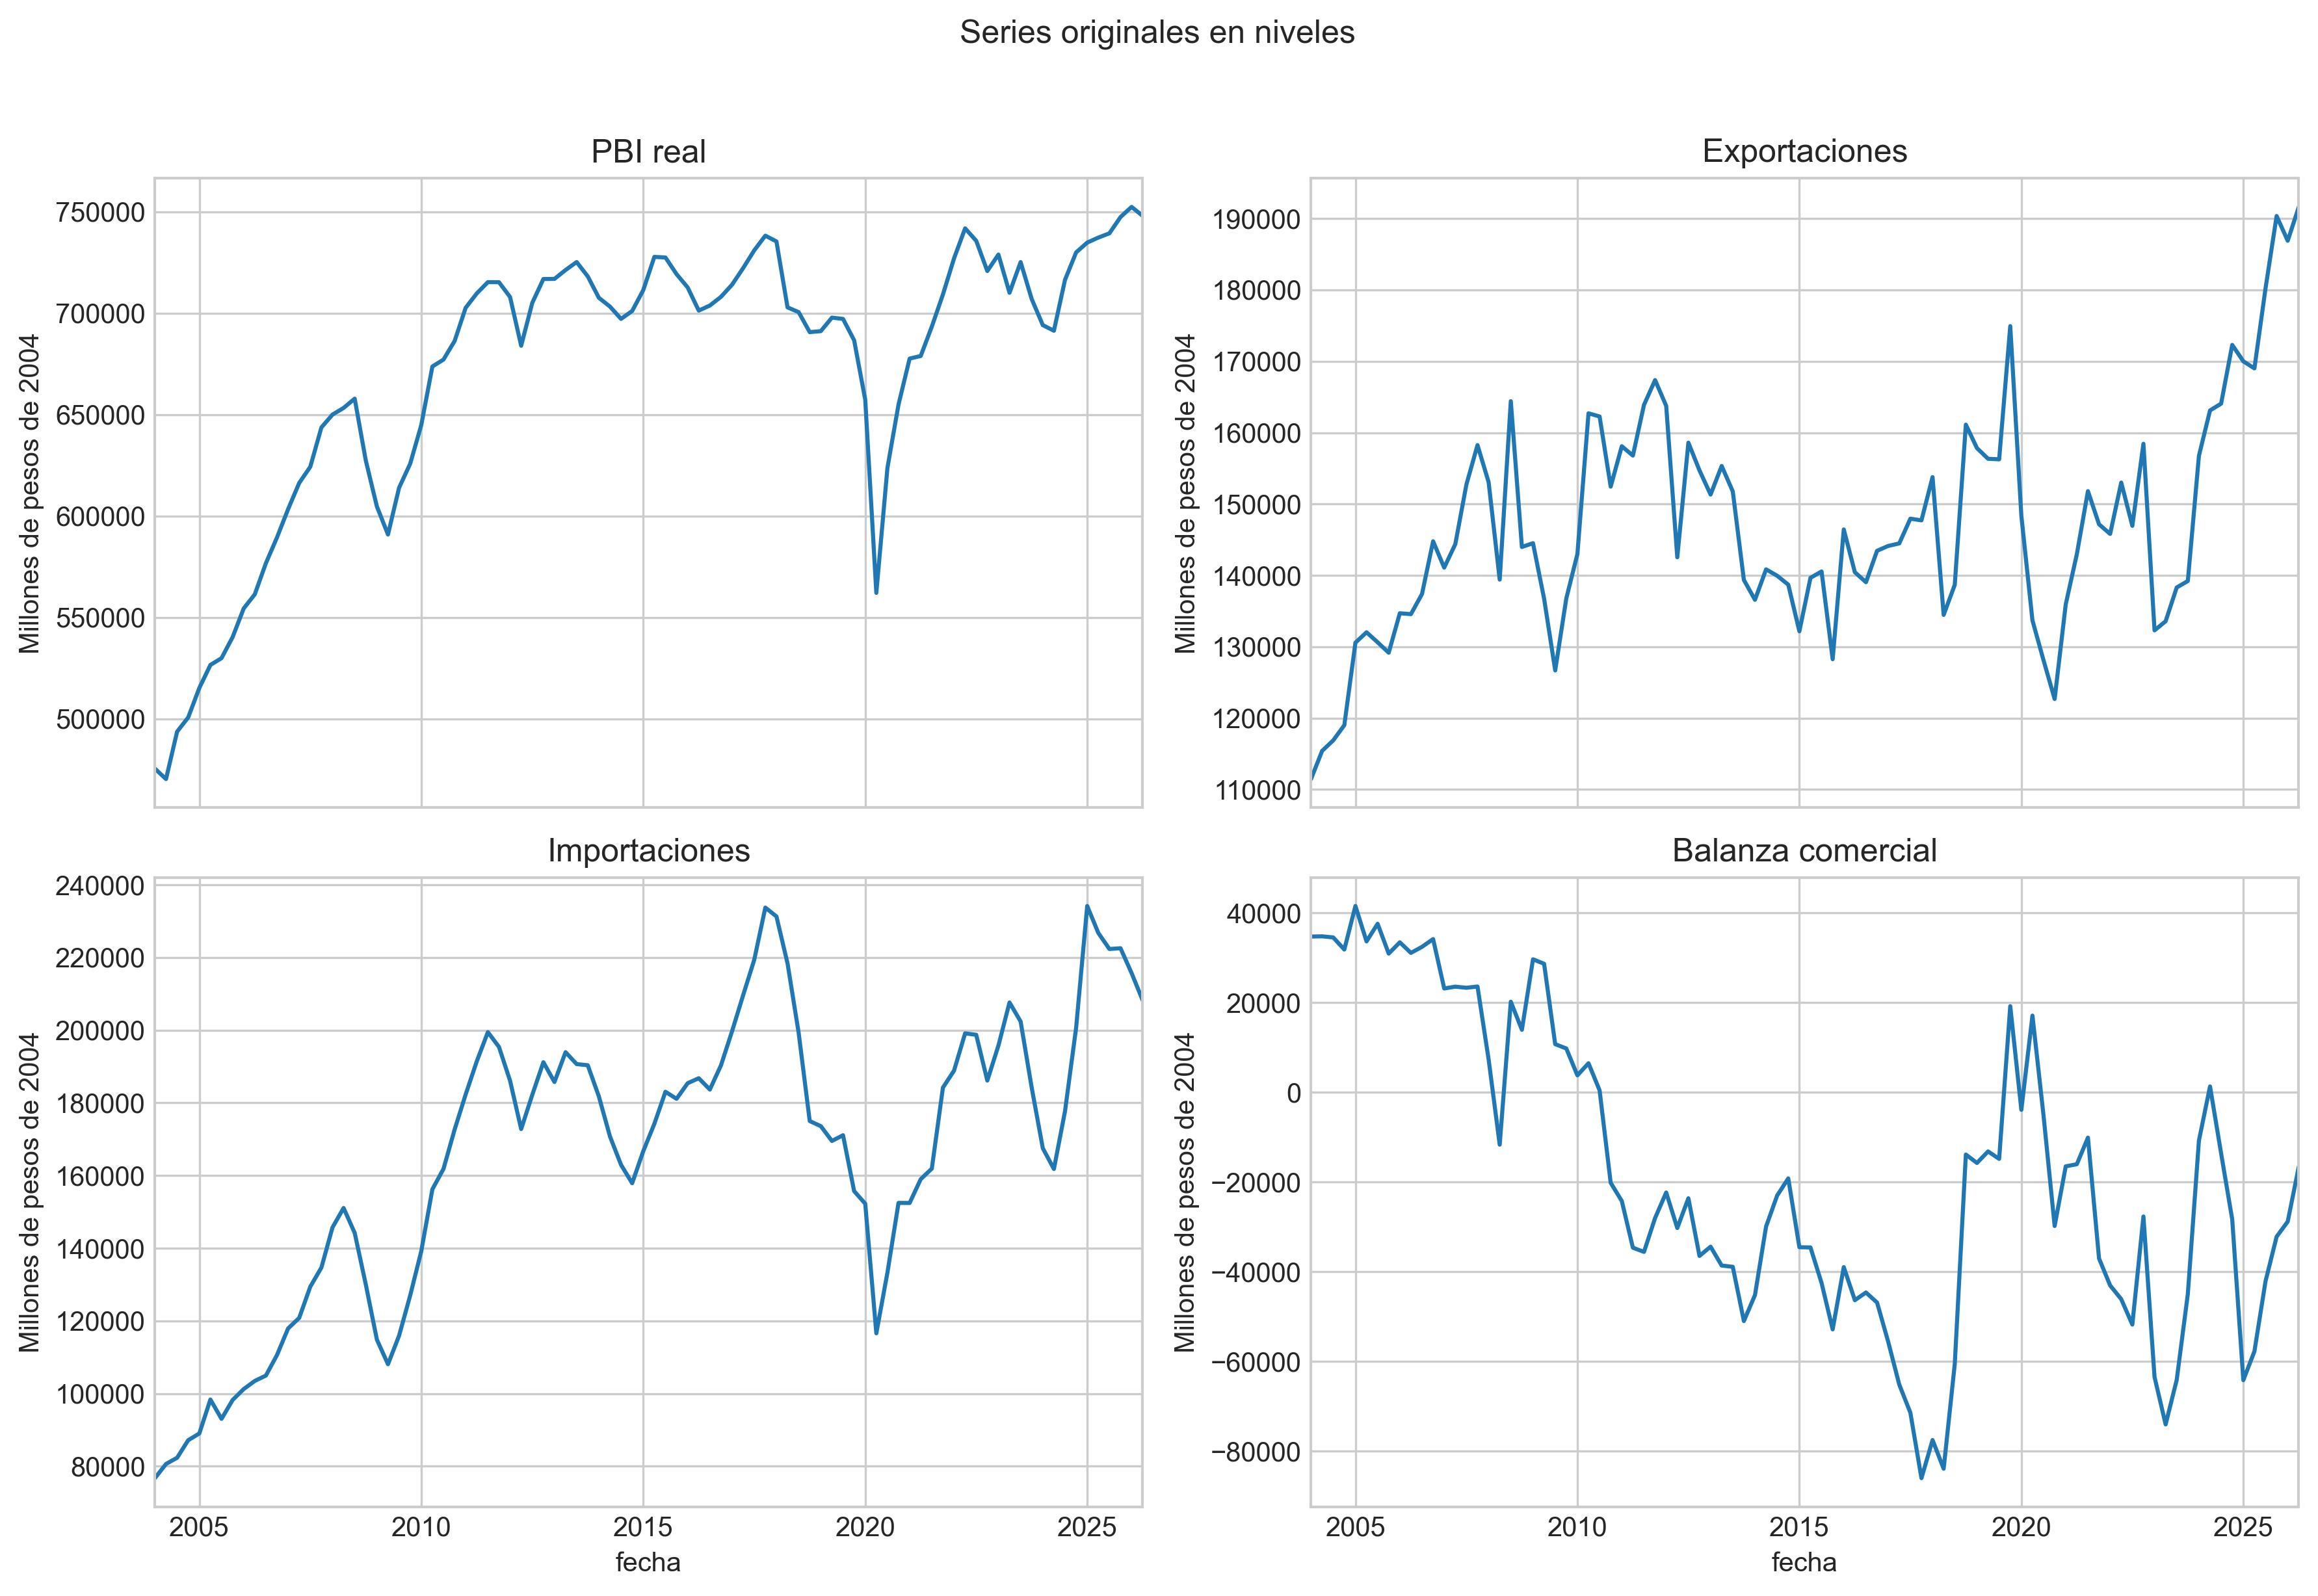
\includegraphics[width=0.92\textwidth]{../results/img/series_niveles_originales.png}
\caption{Variables originales en niveles, 2004-I--2026-II.}
\end{figure}

Despus se muestran las primeras diferencias, es decir, los cambios de un
trimestre al siguiente.

\begin{figure}[H]
\centering
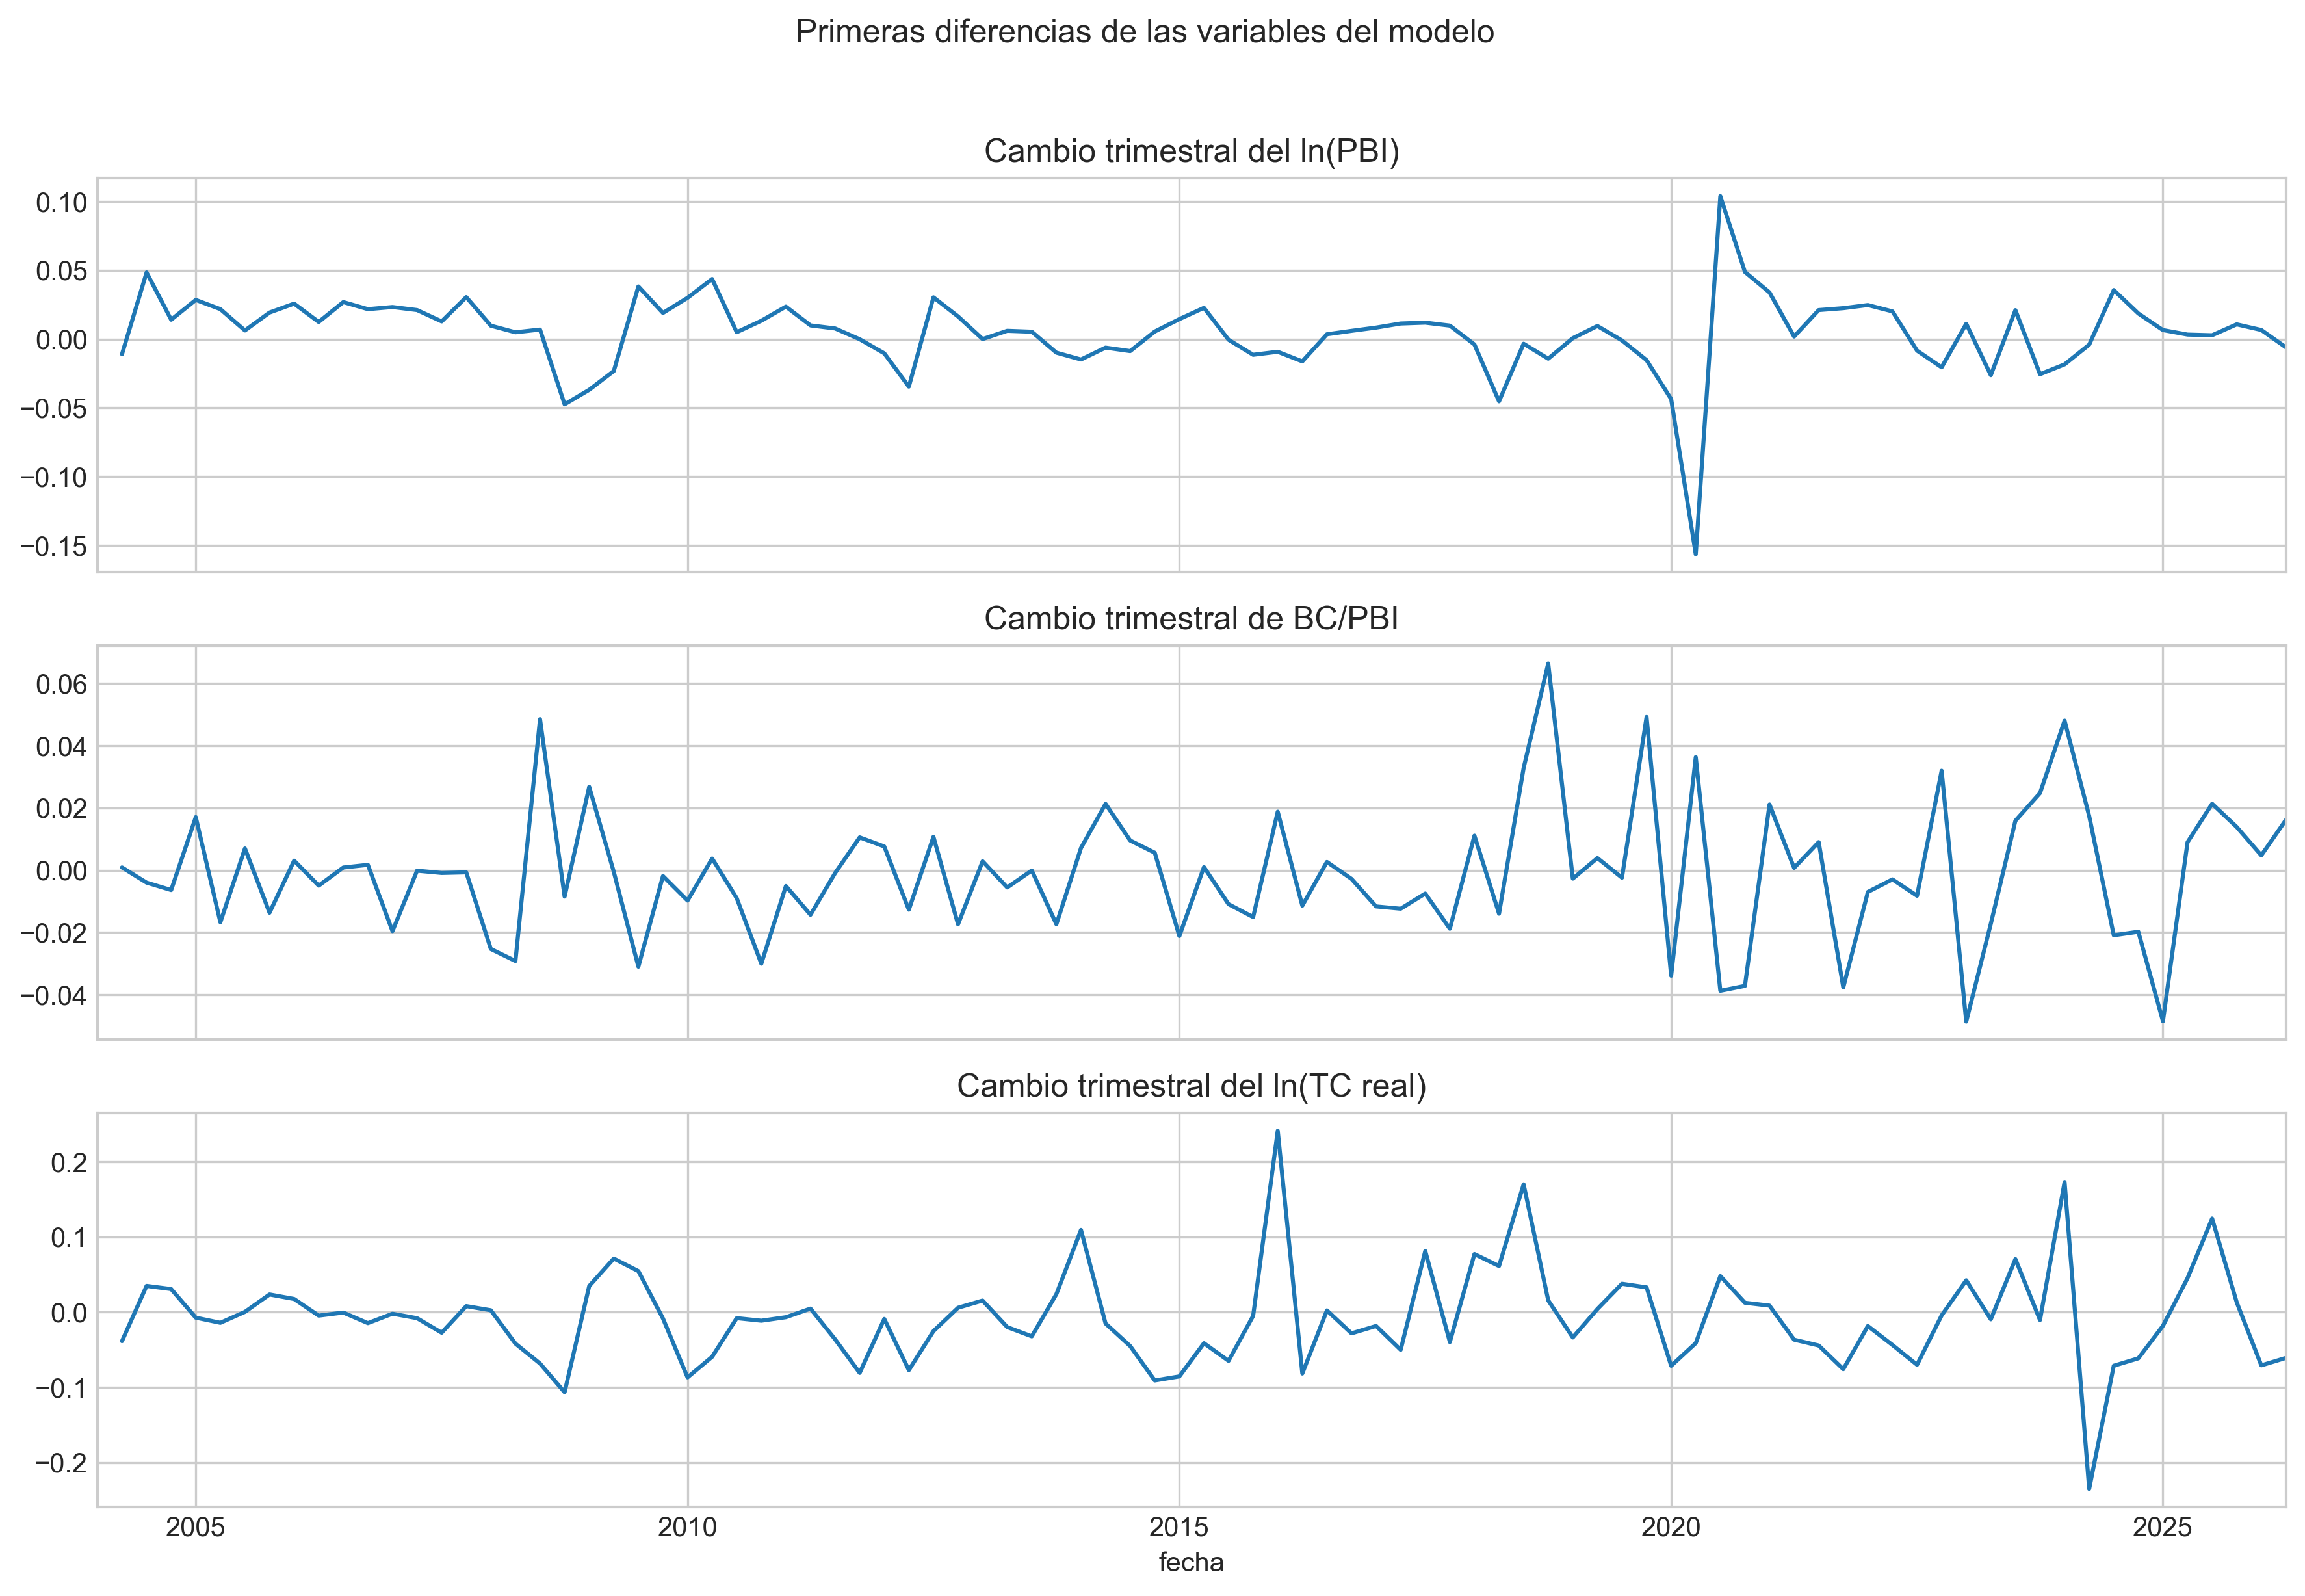
\includegraphics[width=0.92\textwidth]{../results/img/series_primeras_diferencias.png}
\caption{Primeras diferencias de las variables del sistema.}
\end{figure}

\begin{figure}[H]
\centering
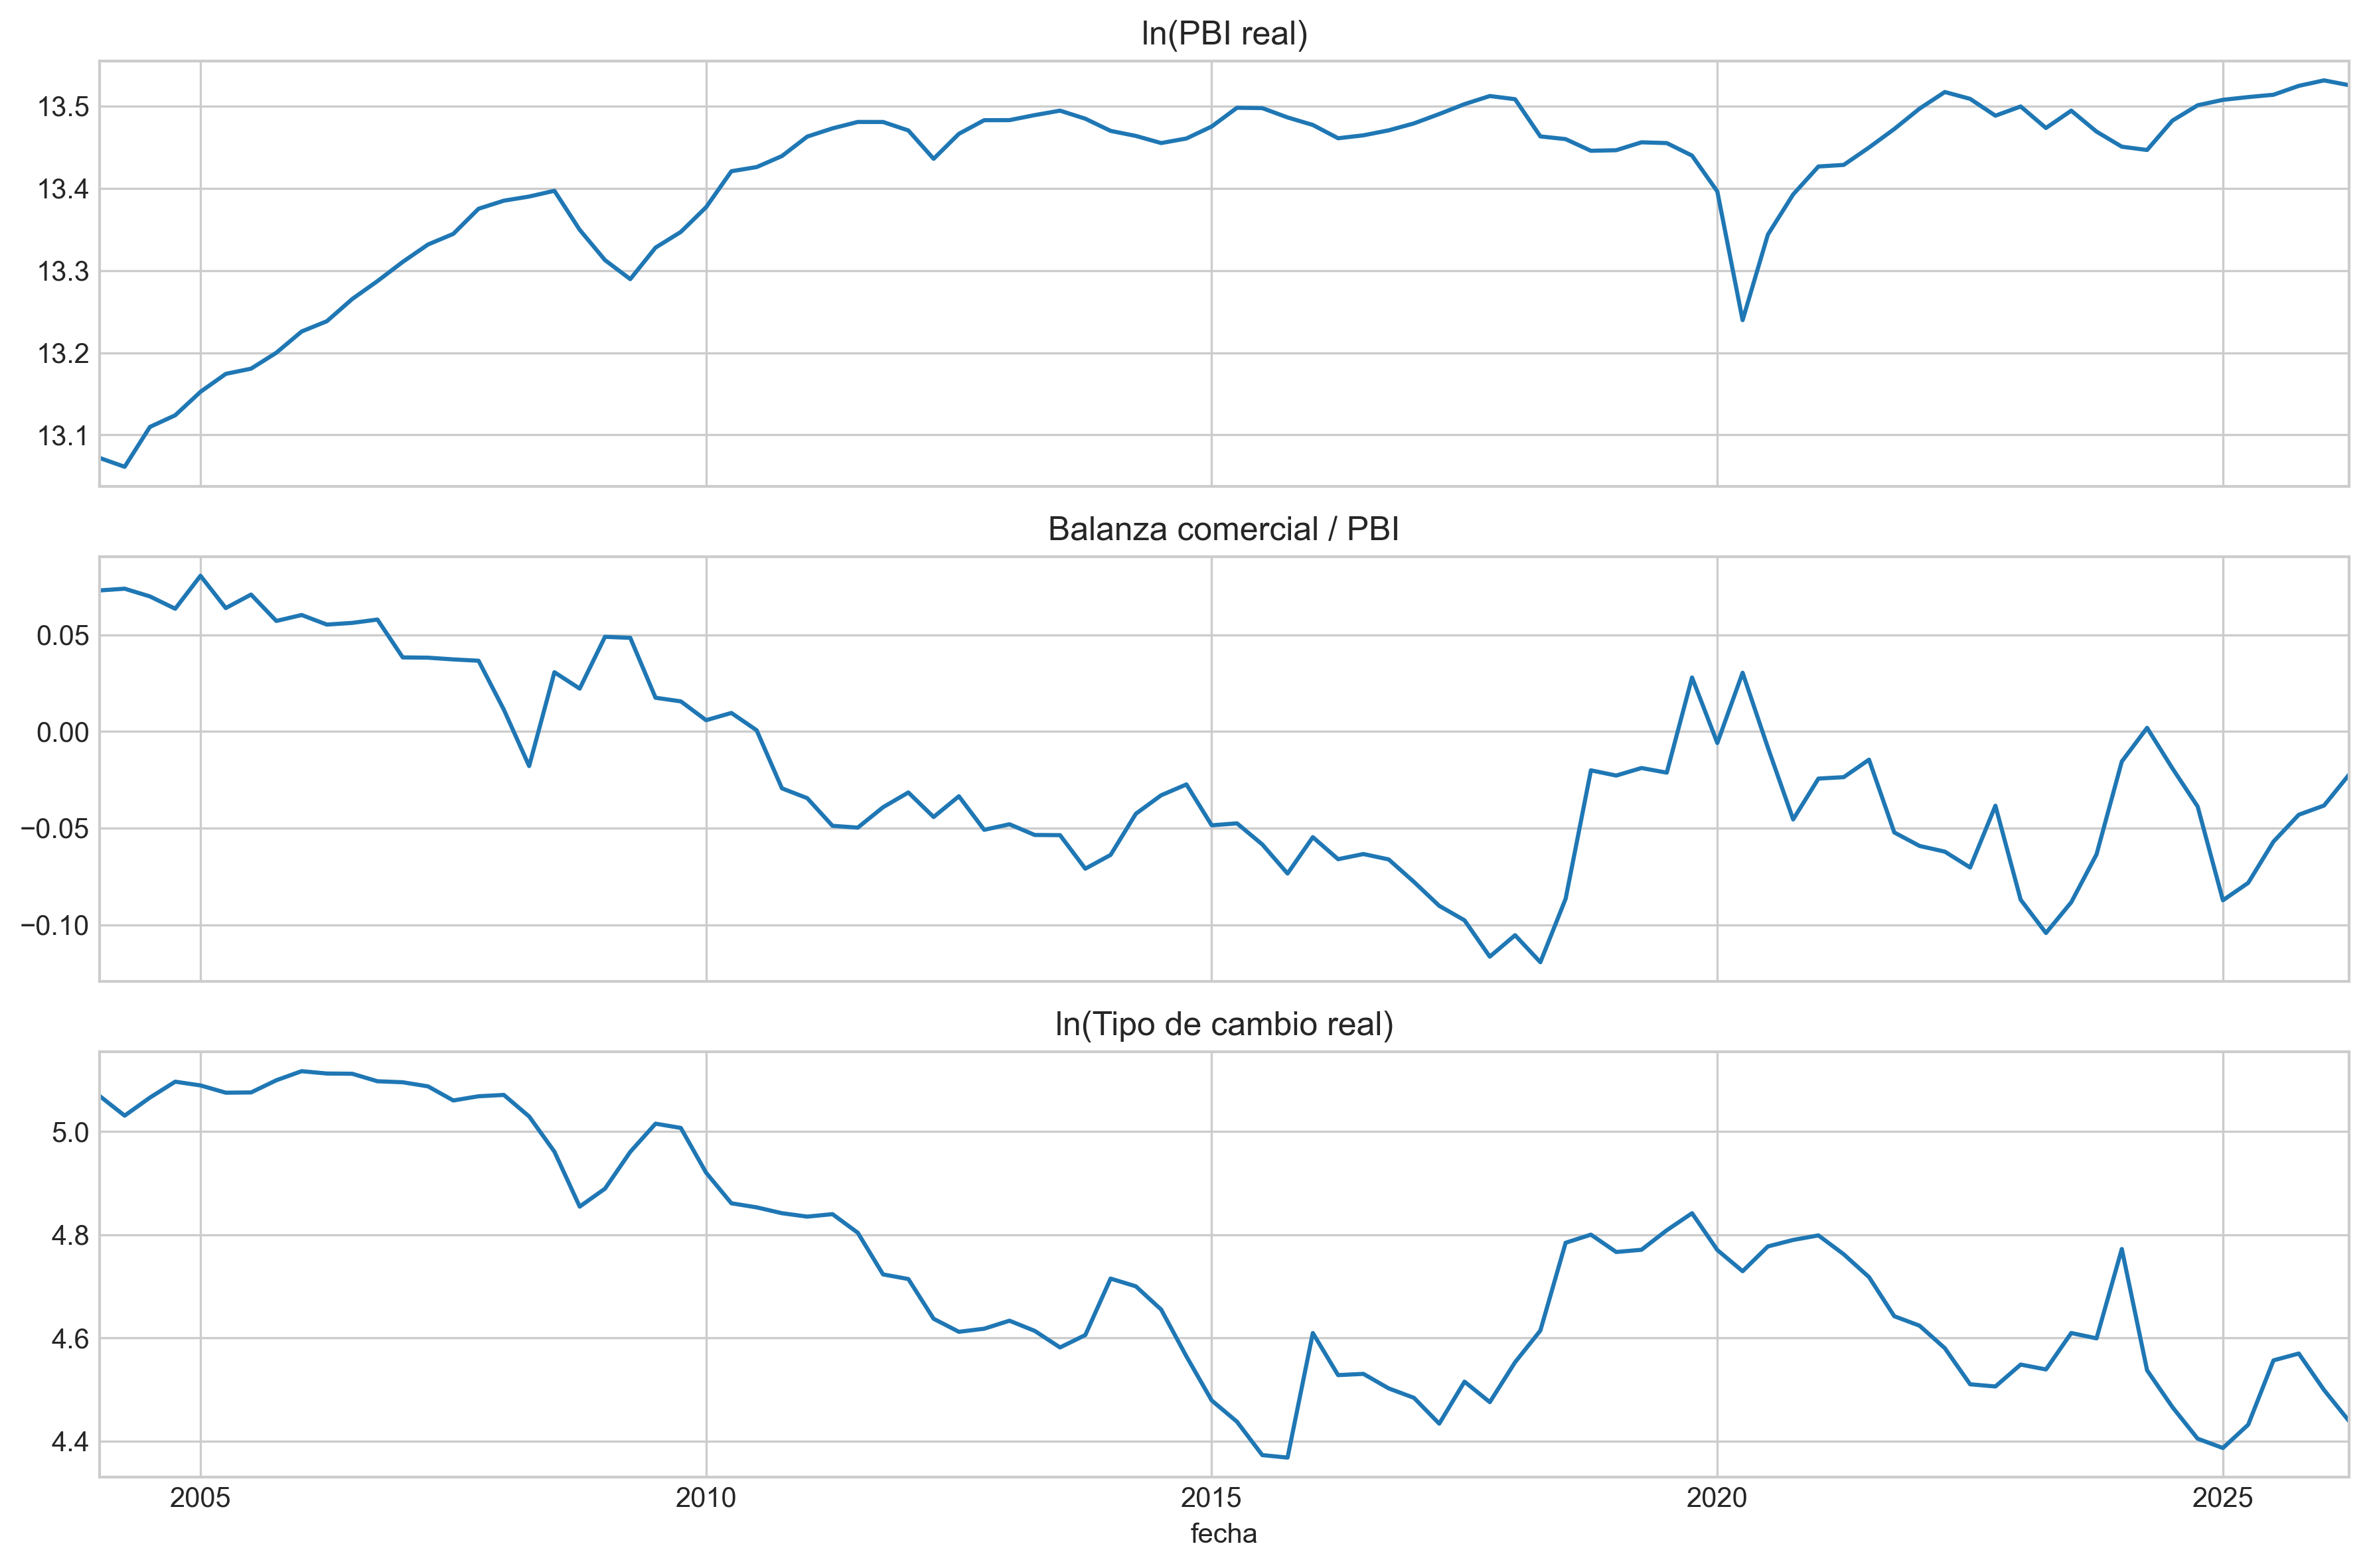
\includegraphics[width=0.92\textwidth]{../results/img/series_modelo.png}
\caption{Variables transformadas utilizadas en el modelo.}
\end{figure}

\begin{figure}[H]
\centering
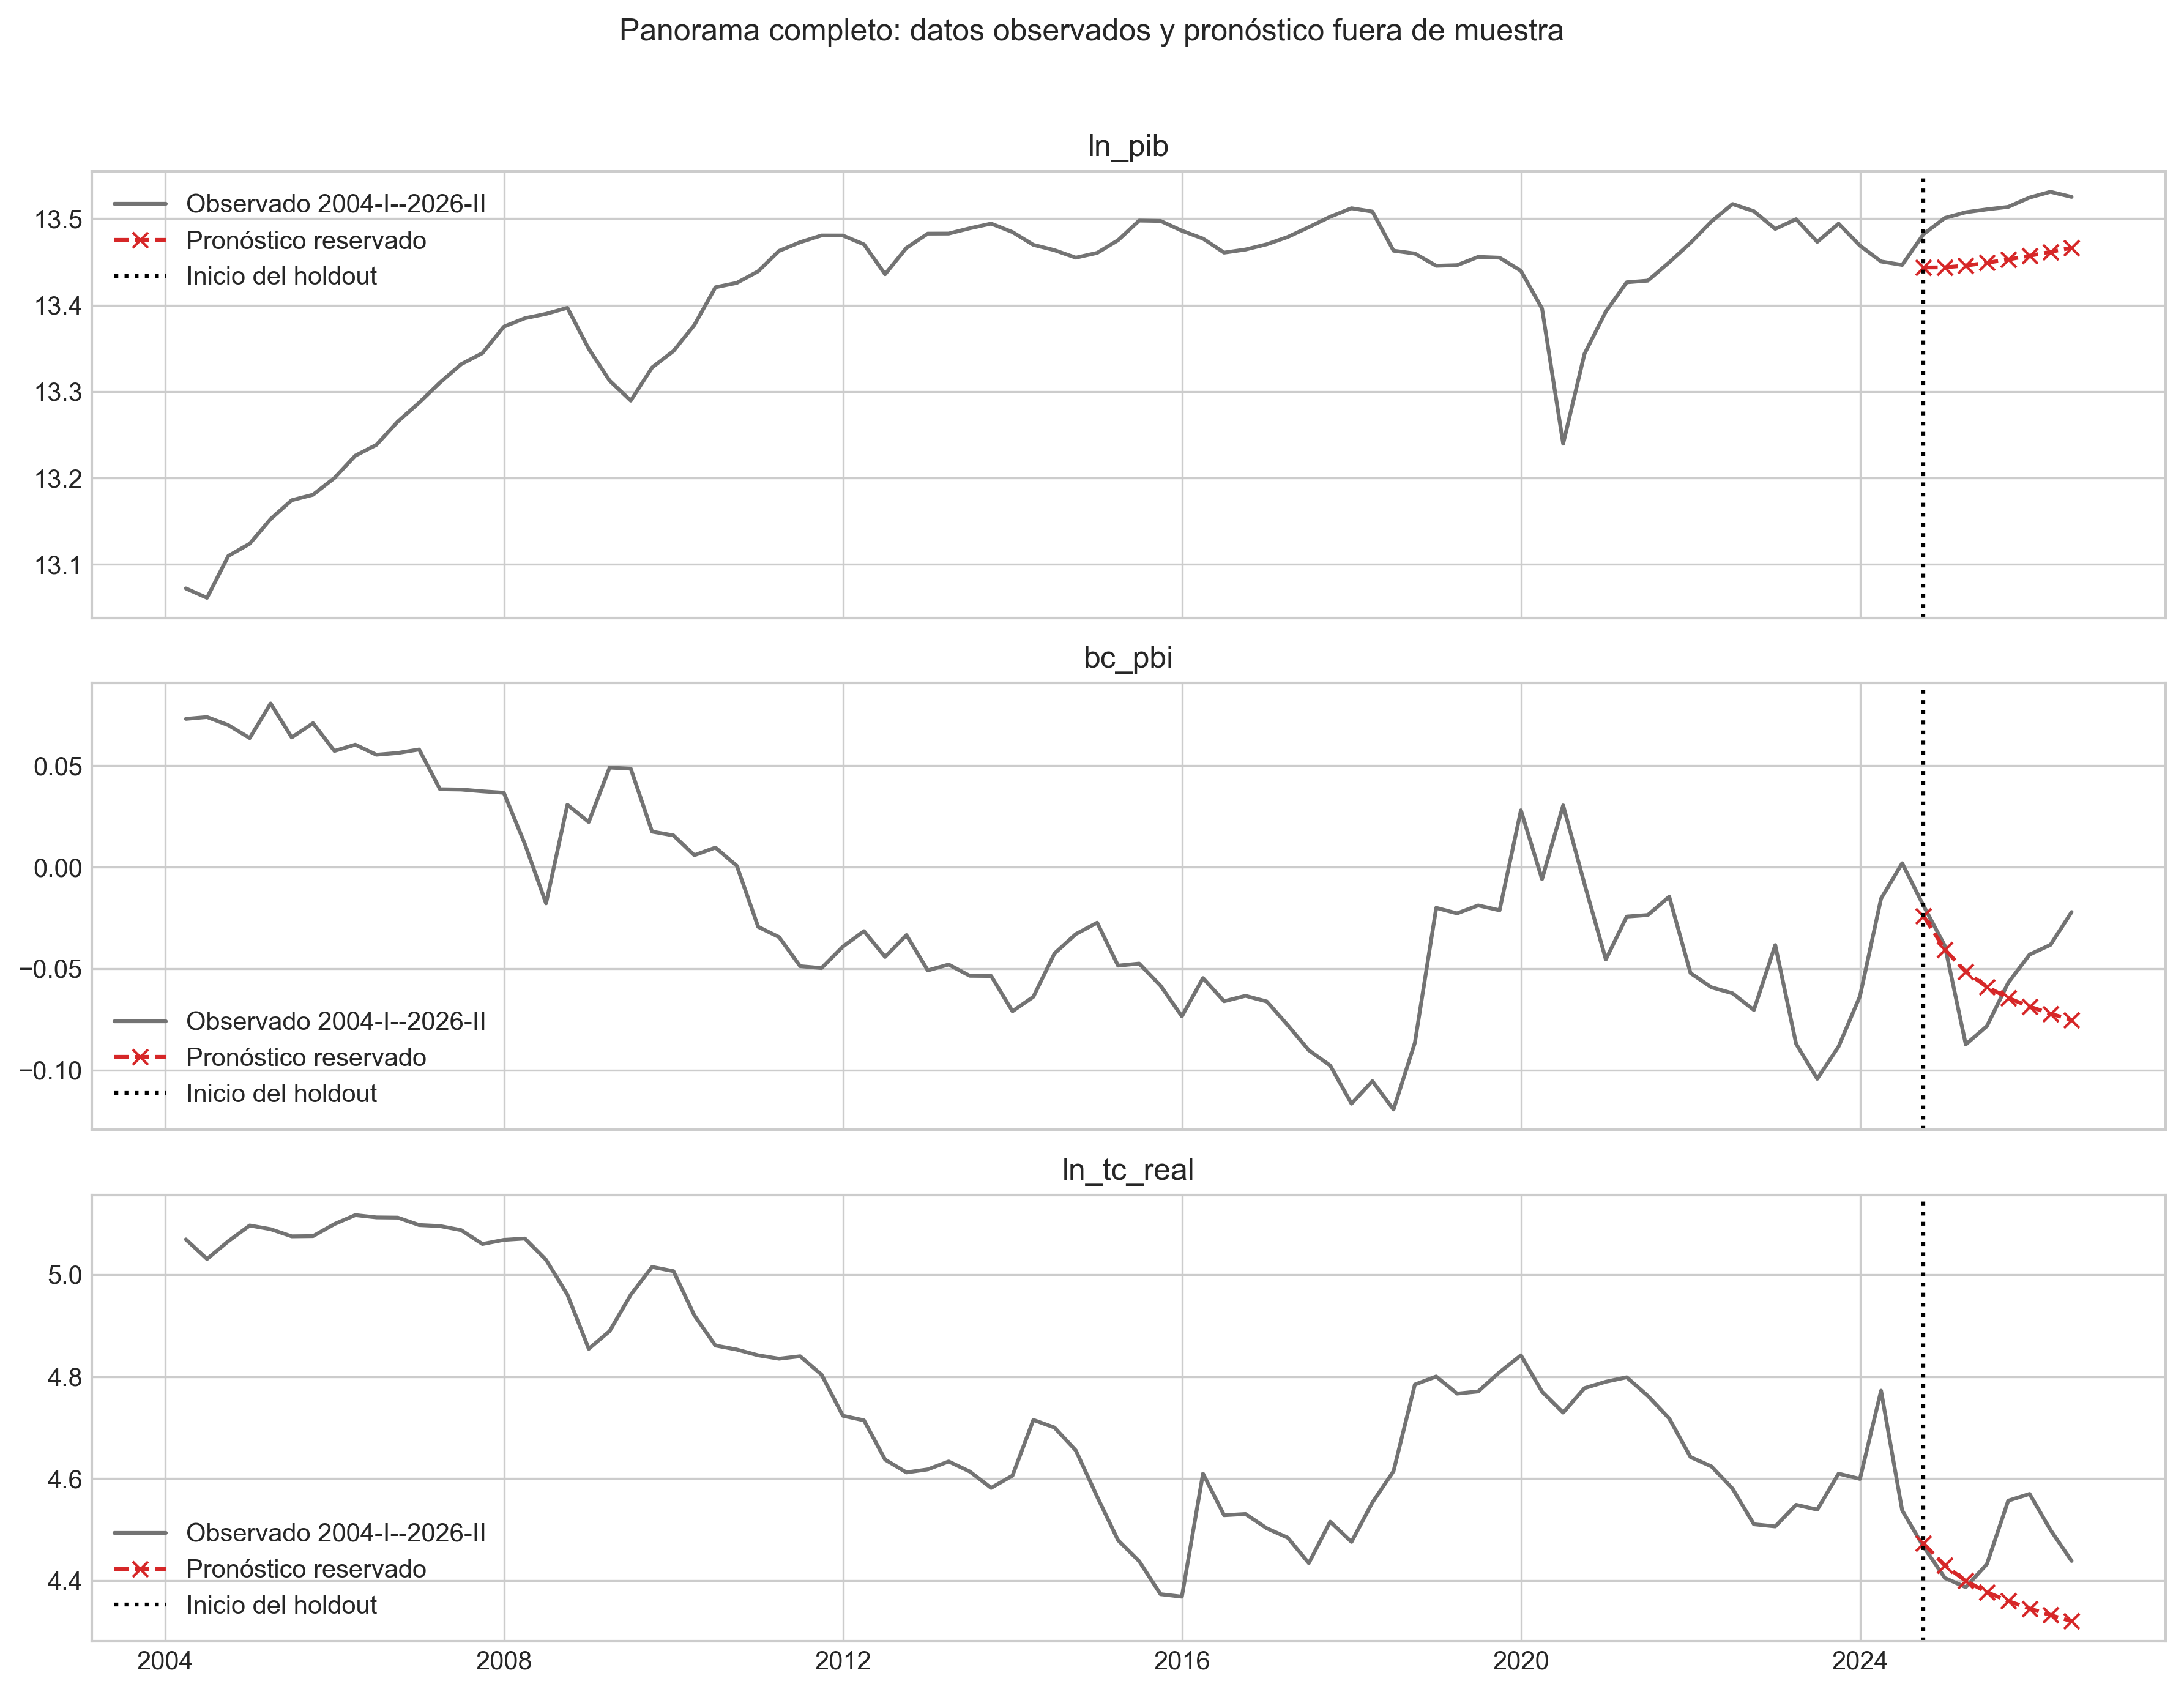
\includegraphics[width=0.92\textwidth]{../results/img/panorama_completo_pronostico.png}
\caption{Datos observados y tramo pronosticado en todo el perodo.}
\end{figure}

\begin{figure}[H]
\centering
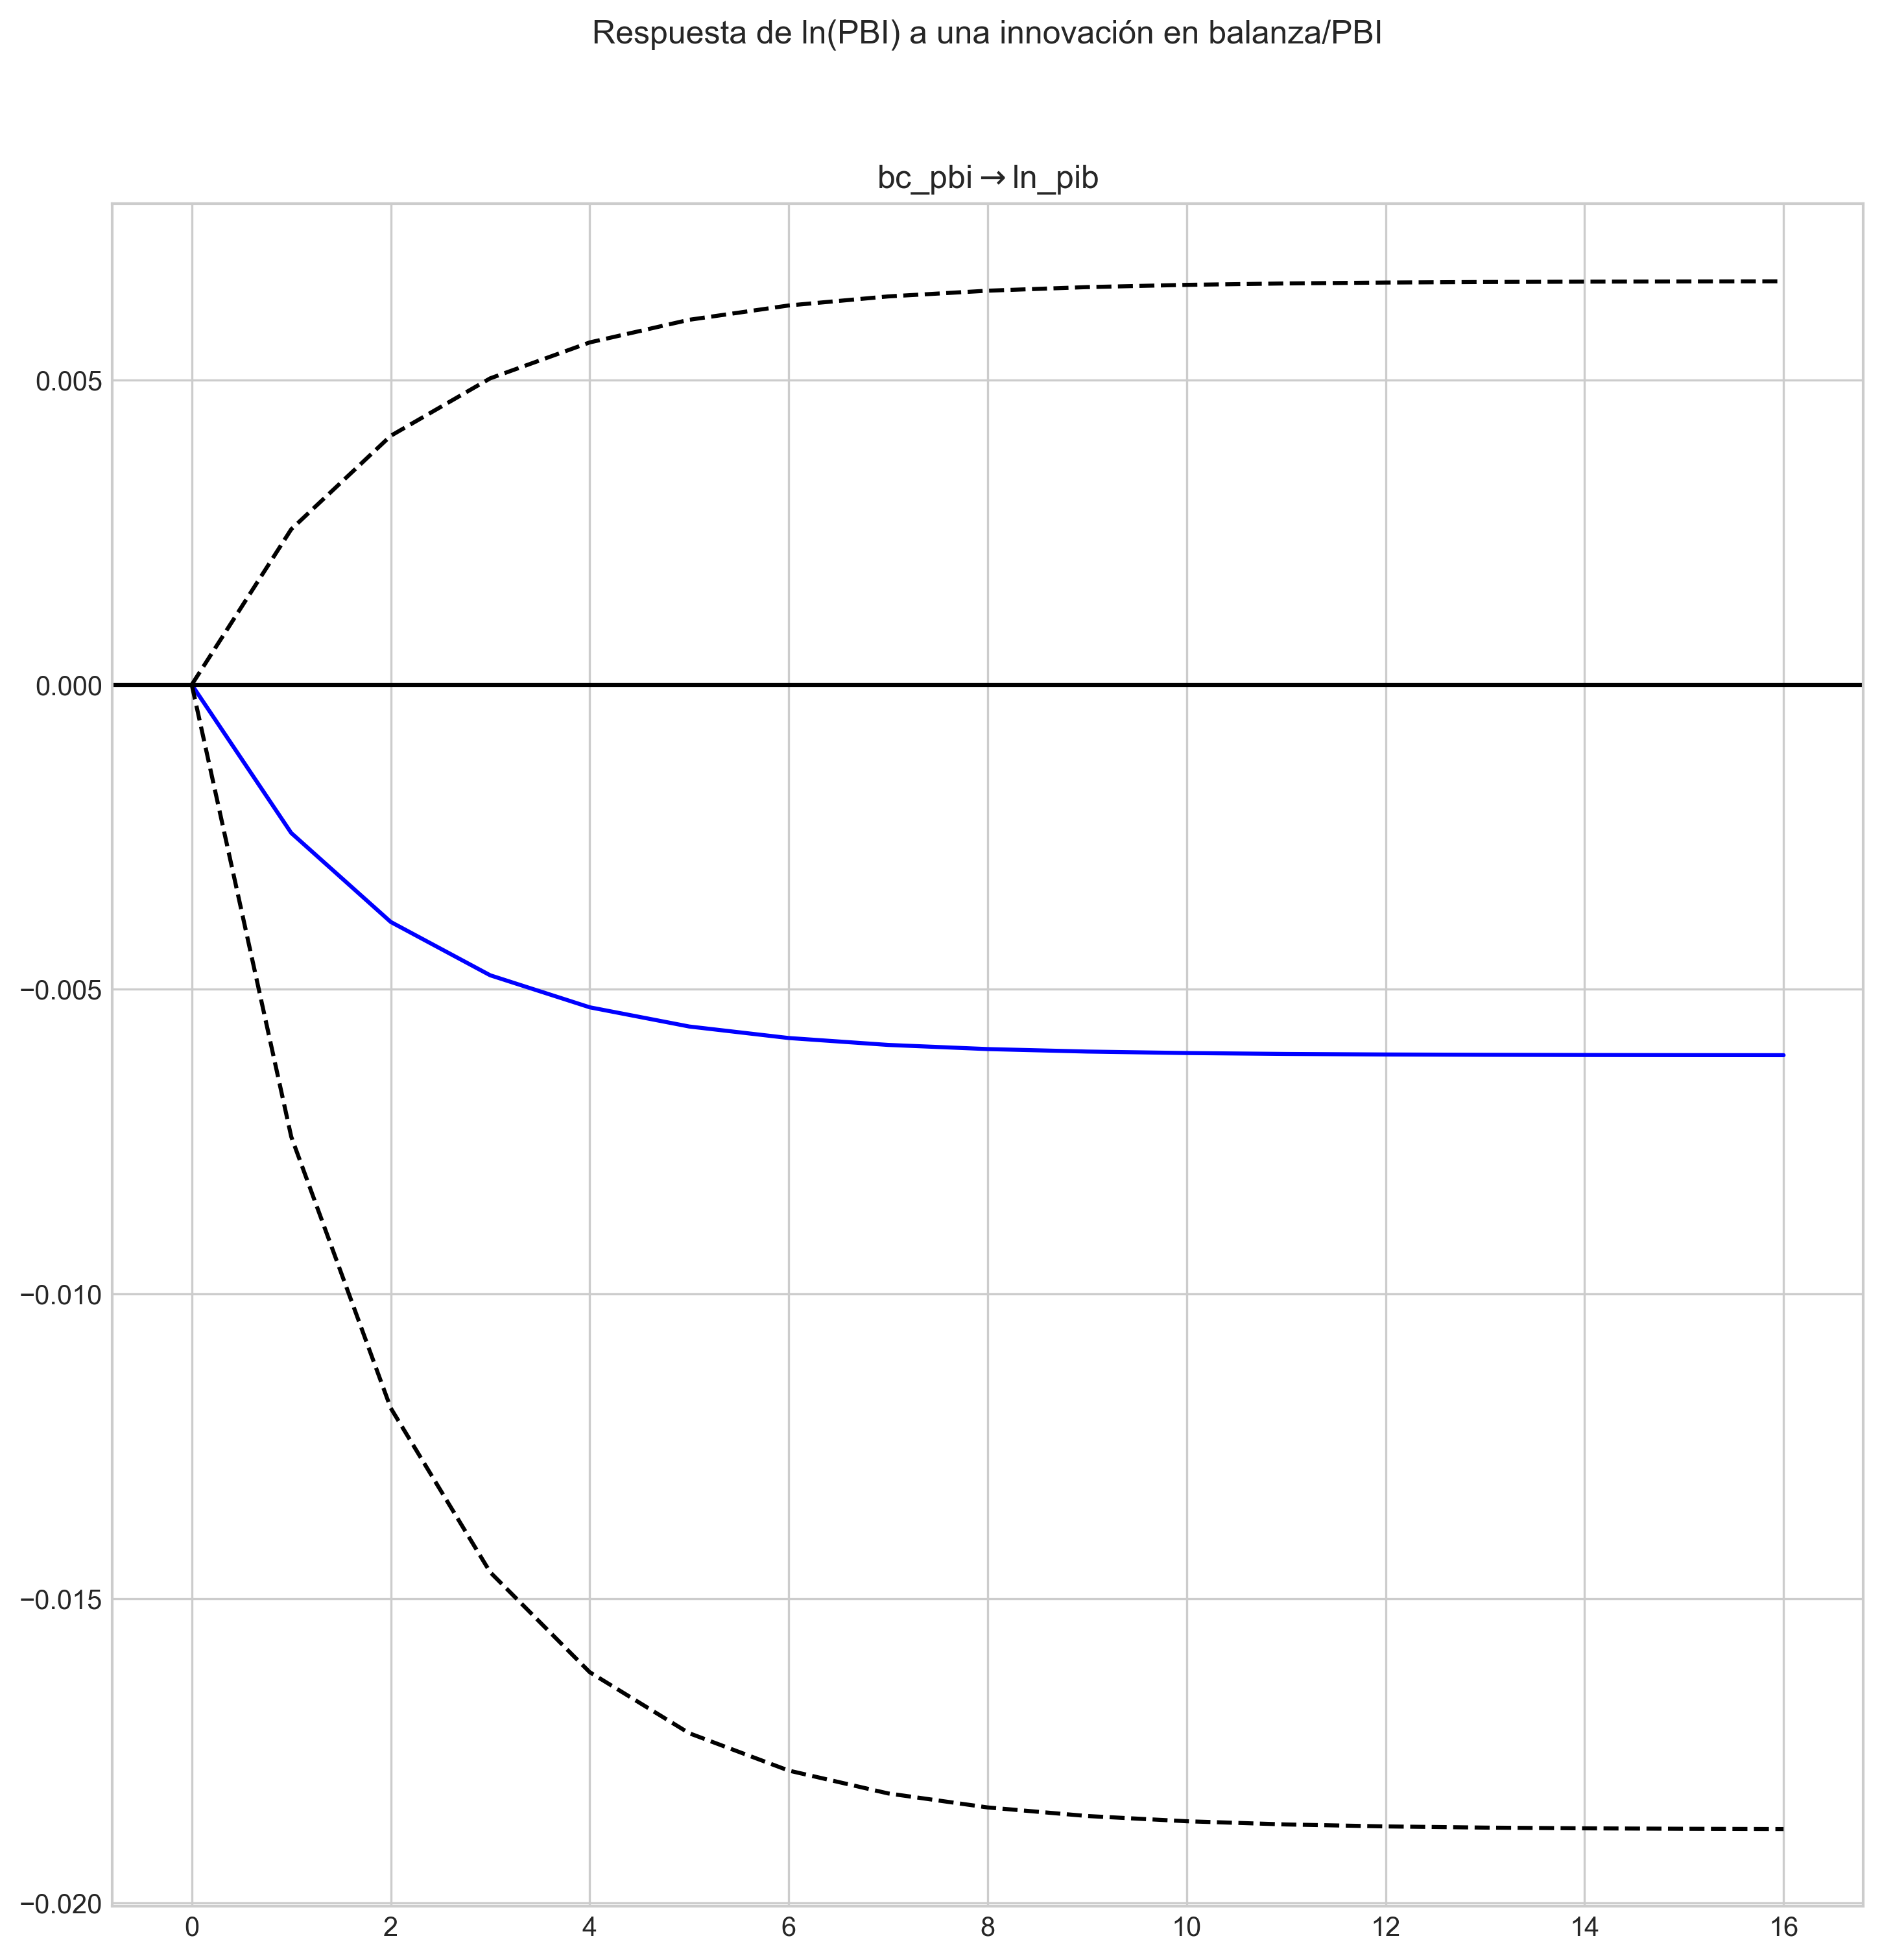
\includegraphics[width=0.92\textwidth]{../results/img/irf_bc_pbi_sobre_pib.png}
\caption{Respuesta del PBI ante una innovacin en la balanza comercial relativa.}
\end{figure}

\begin{figure}[H]
\centering
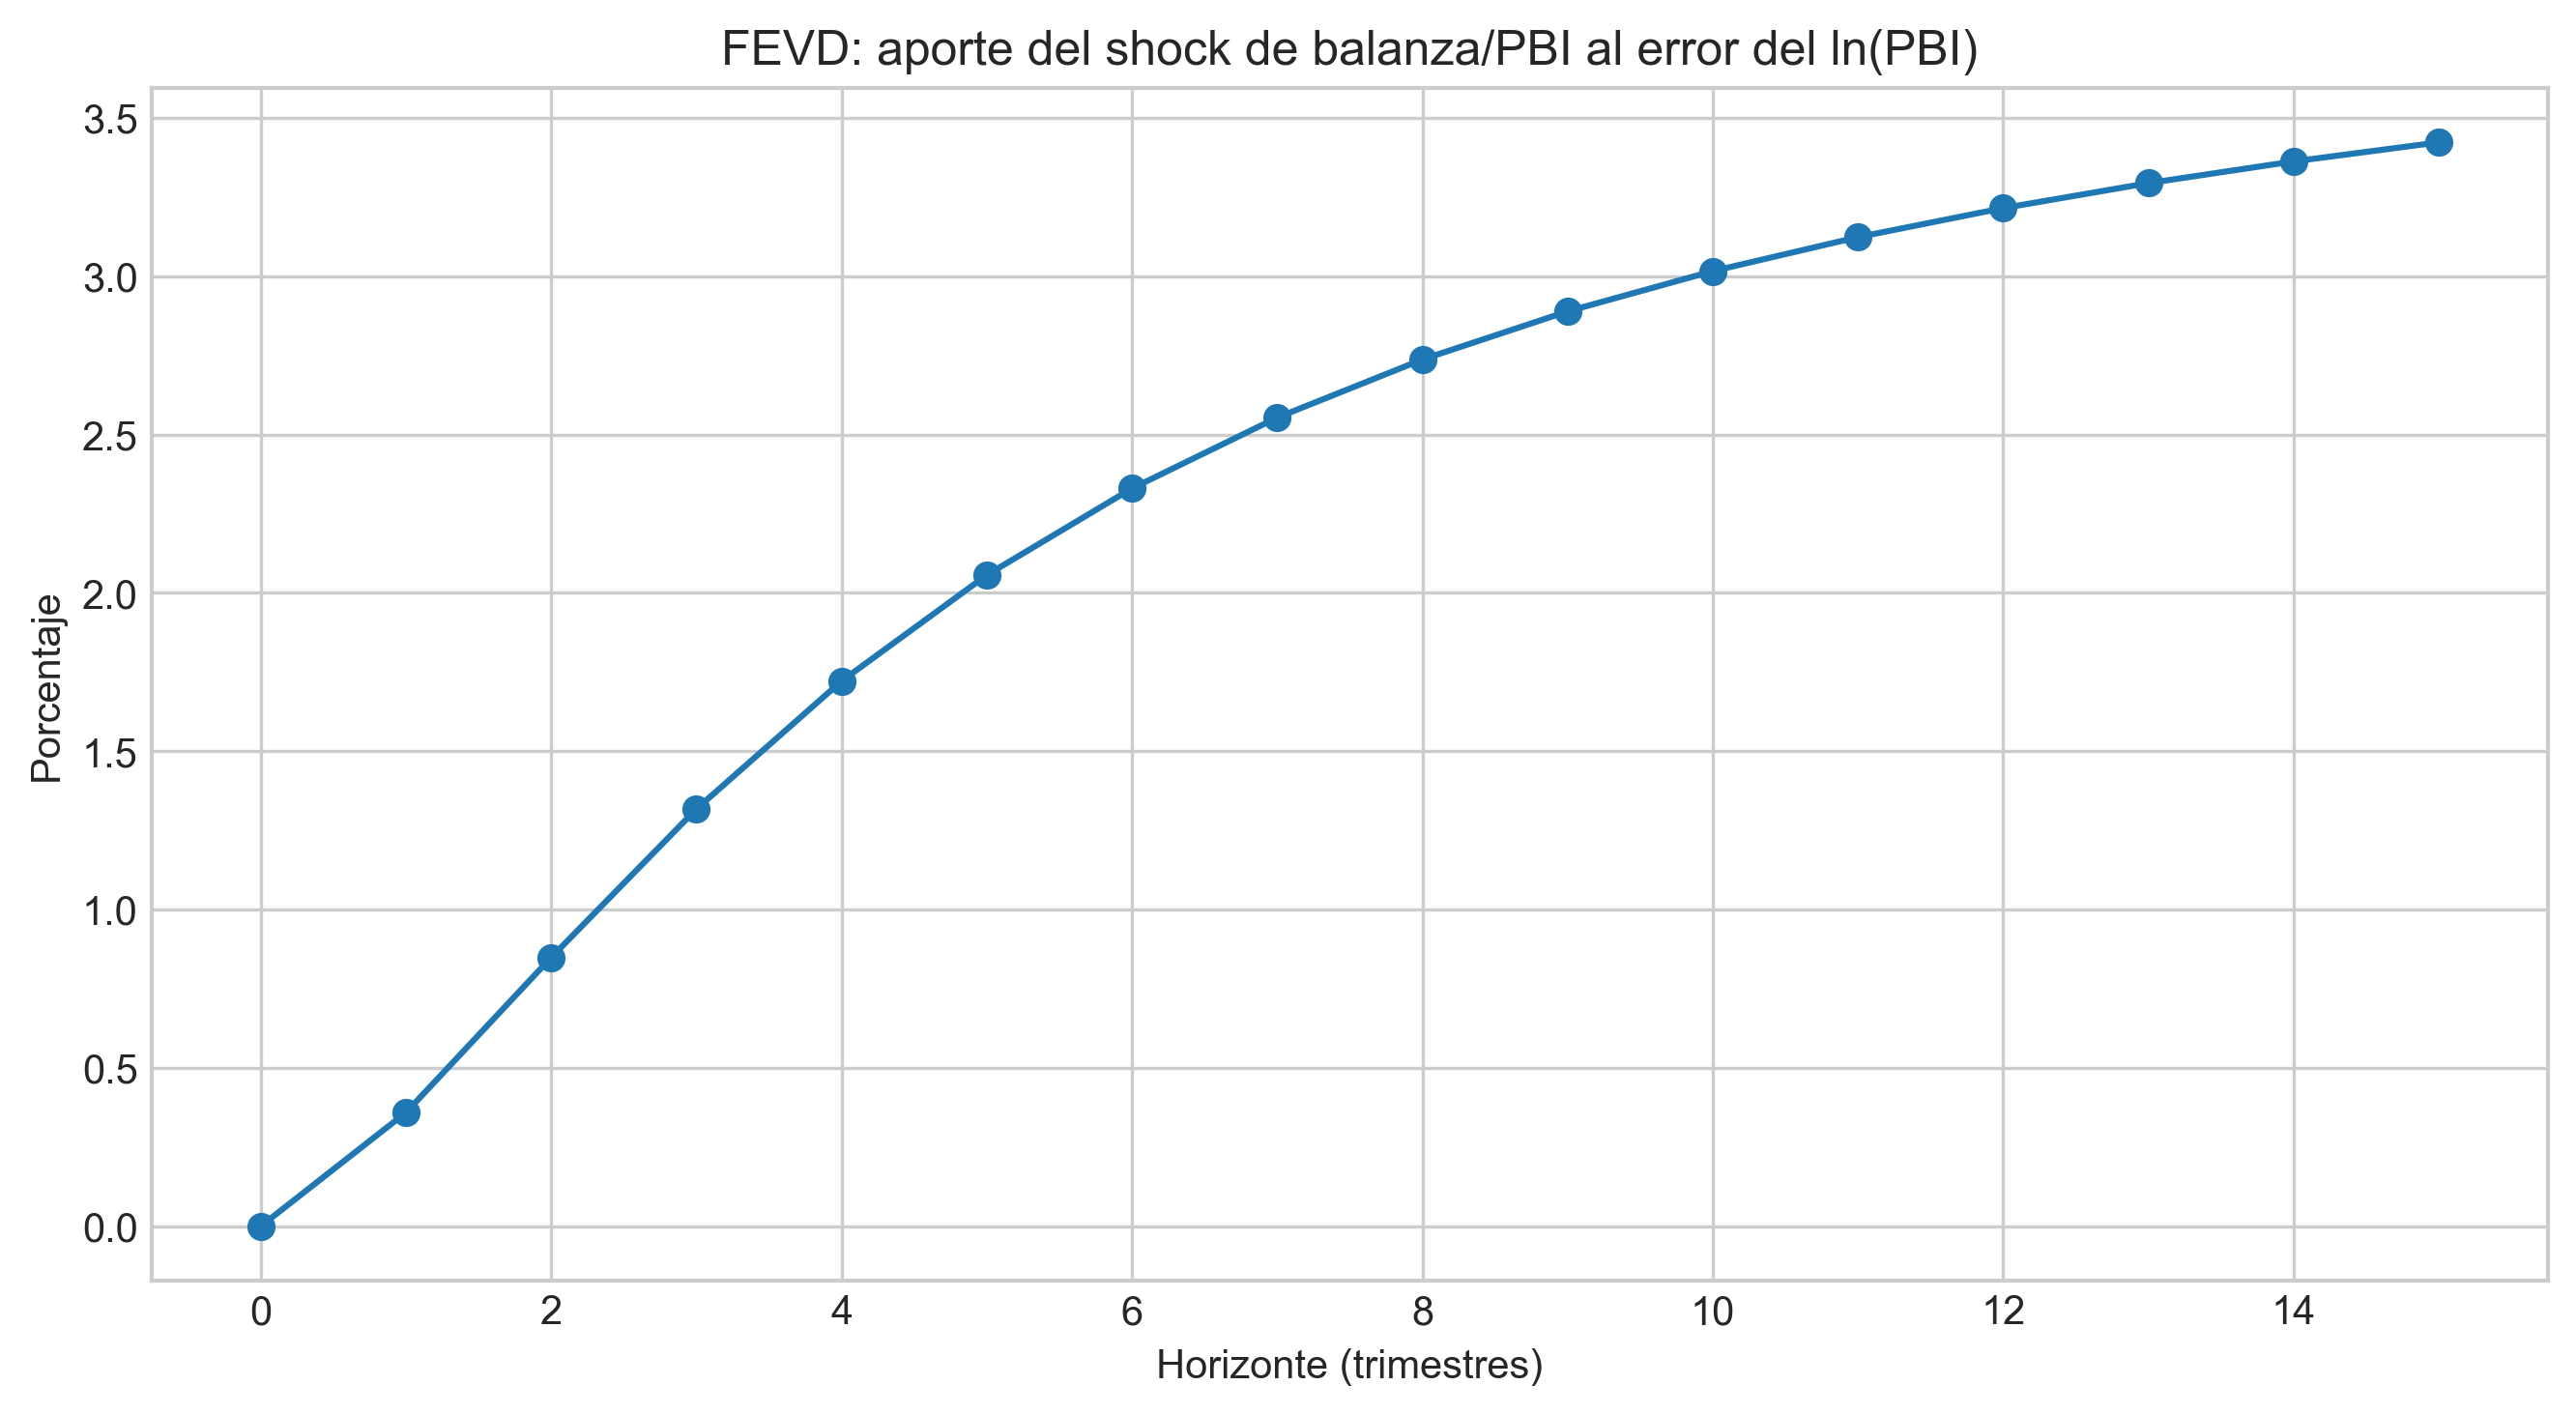
\includegraphics[width=0.92\textwidth]{../results/img/fevd_bc_pbi_sobre_pib.png}
\caption{Aporte del shock de la balanza al error de pronstico del PBI.}
\end{figure}

\section{Evaluacion fuera de muestra}

Para comprobar el desempeno predictivo se reservo el periodo 2024-III--2026-II
sin utilizarlo para seleccionar rezagos, aplicar Johansen ni estimar el modelo.
Los pronosticos
y los valores observados se encuentran en
\texttt{results/pronostico\_holdout.csv}.

\begin{figure}[H]
\centering
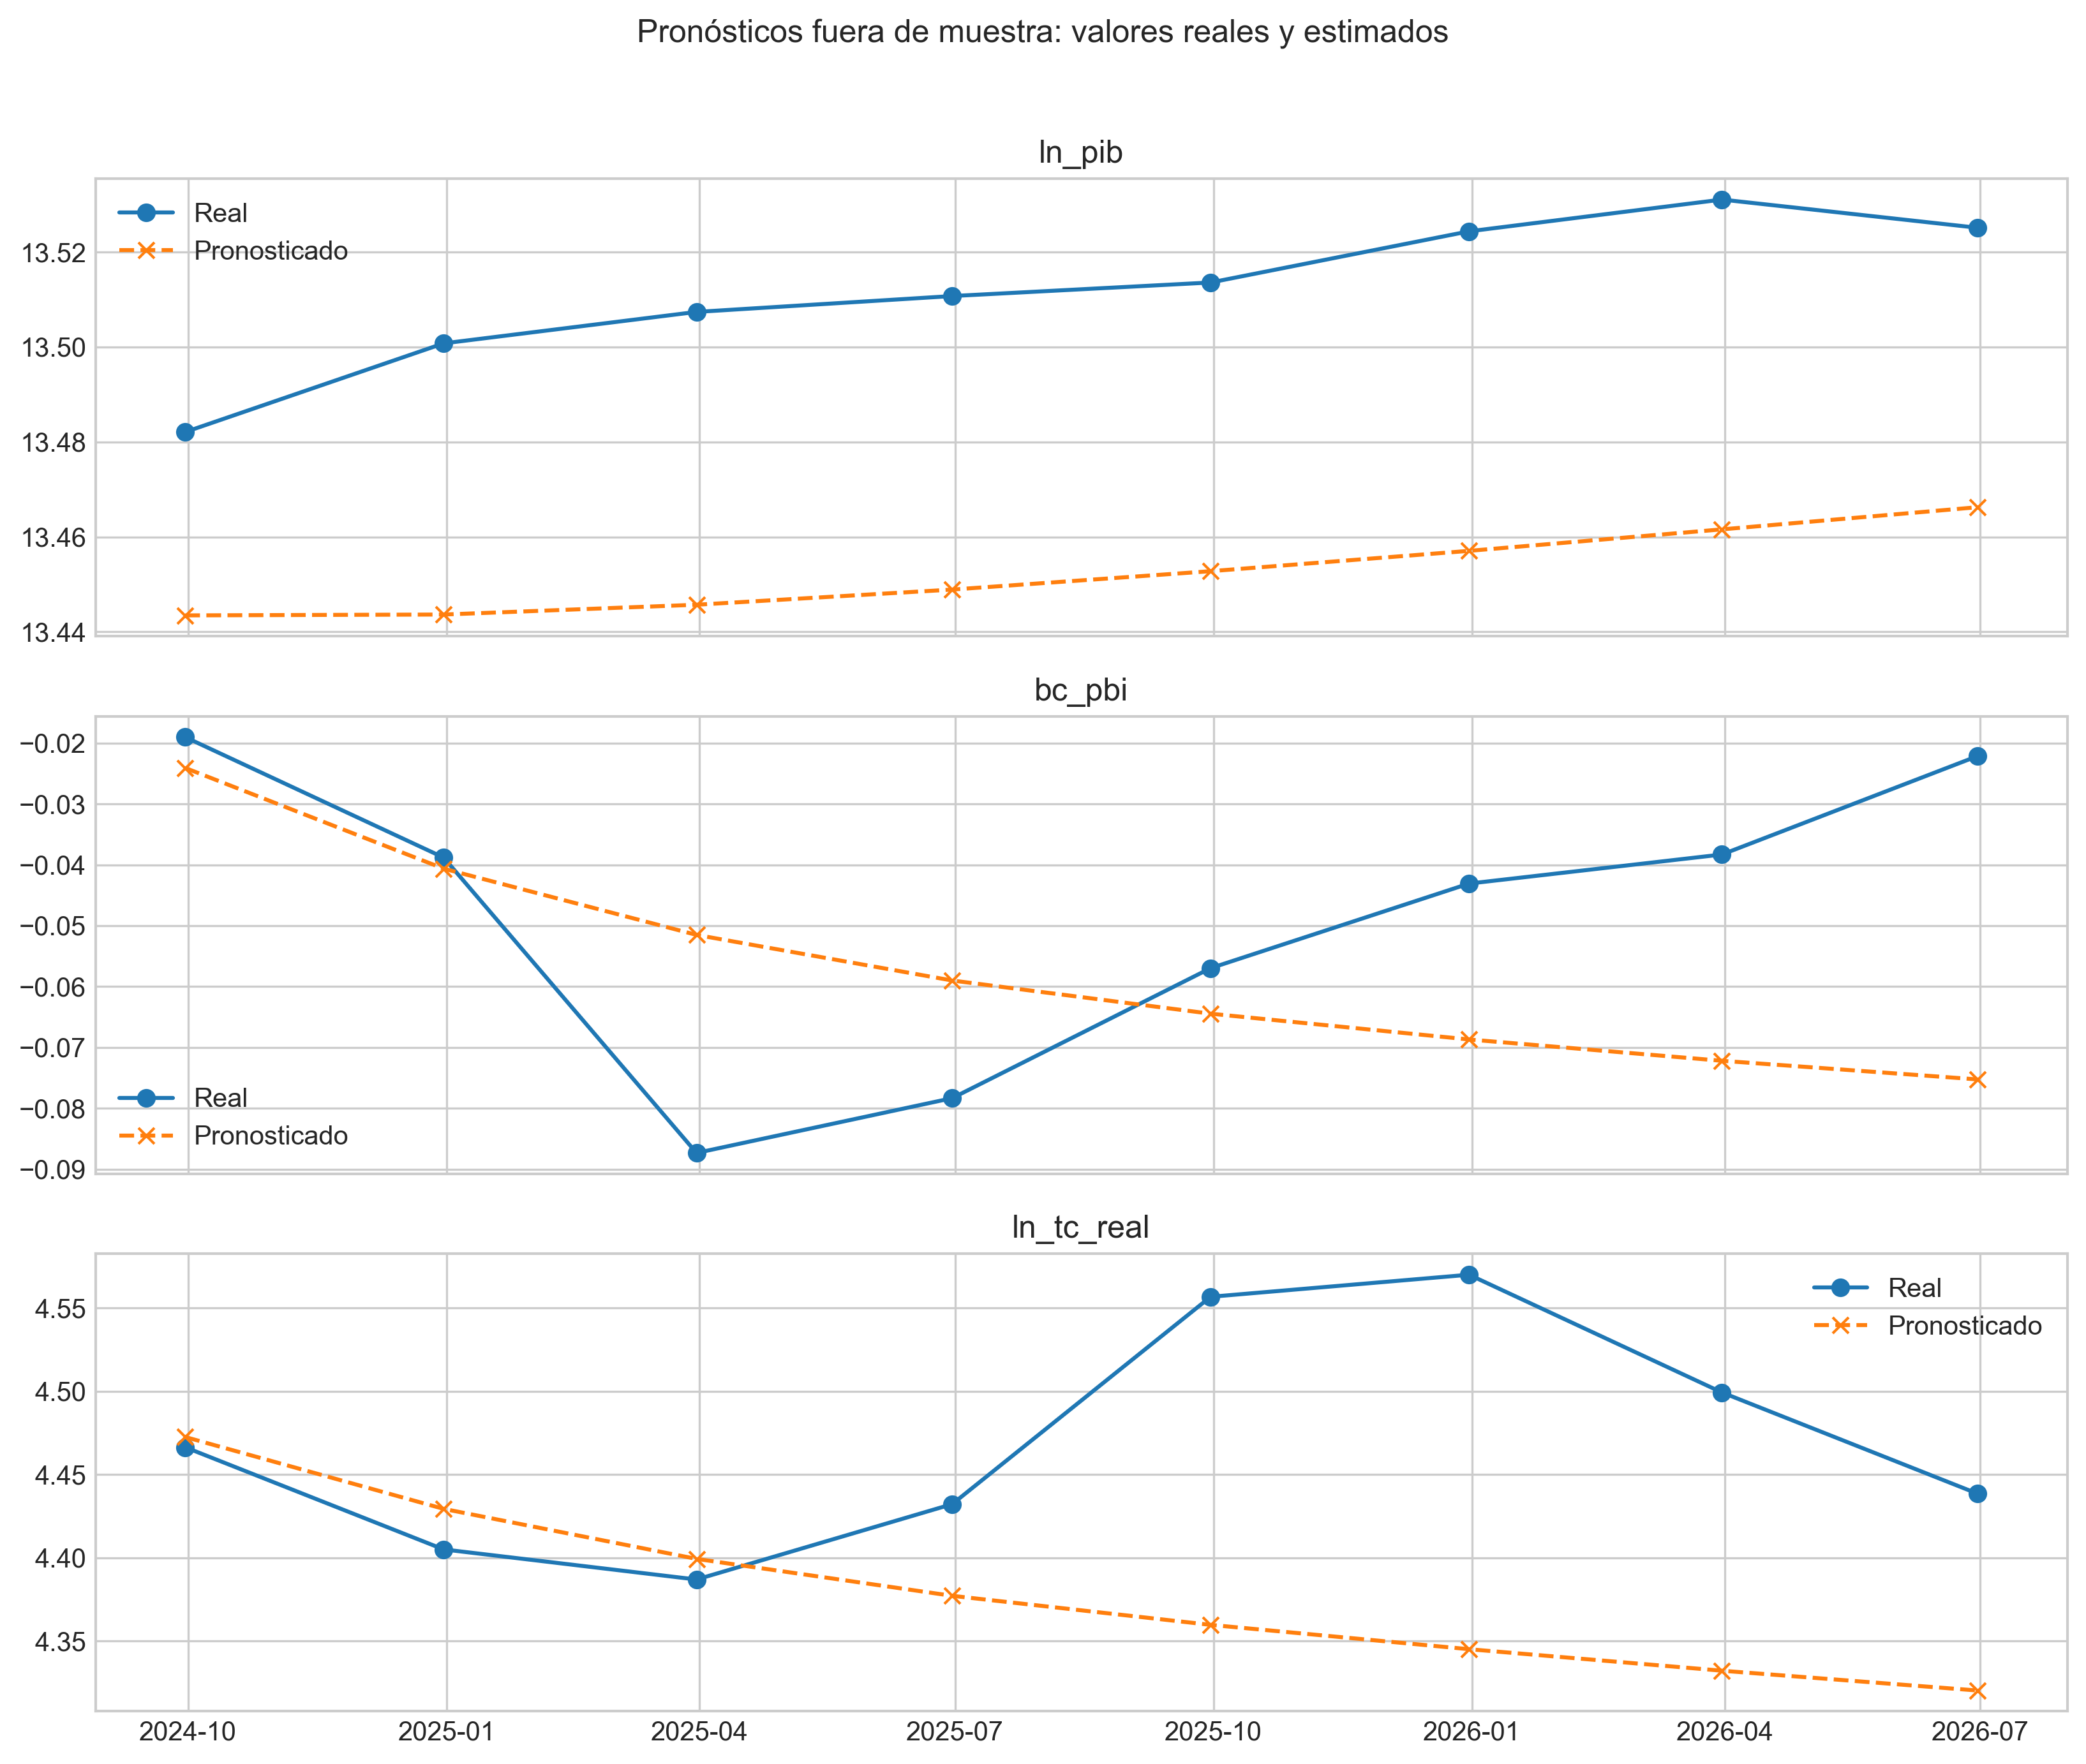
\includegraphics[width=0.92\textwidth]{../results/img/pronostico_real_vs_estimado.png}
\caption{Valores observados y pronosticados en la muestra reservada.}
\end{figure}

El RMSE y el MAE de $\ln(PBI)$ fueron 0.0601 y 0.0595, respectivamente. Para
$\ln(TC\ real)$ fueron 0.1299 y 0.1006. Para $BC/PBI$ fueron 0.0282 y 0.0228.
El MAPE de $BC/PBI$ fue 62.26\% y no debe utilizarse como criterio principal
porque esta variable puede acercarse a cero y cambiar de signo; por esa razon
se priorizan RMSE y MAE. Los resultados completos estan en
\texttt{results/metricas\_pronostico.csv}.

\section{Archivos reproducibles}

Los principales resultados se guardan en la carpeta \texttt{results}:
\texttt{data\_modelo\_completa.csv}, \texttt{data\_modelo\_entrenamiento.csv},
\texttt{data\_modelo\_rezagos.csv}, \texttt{pronostico\_holdout.csv},
\texttt{metadatos\_modelo.csv}, \texttt{pruebas\_raiz\_unitaria.csv},
\texttt{cointegracion\_johansen.csv}, \texttt{diagnostico\_cusum.csv} y
\texttt{resumen\_modelo.tex}. El resumen legible de las pruebas se encuentra en
\texttt{resumen\_pruebas.txt}. Las figuras se ubican en
\texttt{results/img}.

\section{Fuentes institucionales}

\begin{itemize}[leftmargin=*]
  \item INDEC, comercio exterior:
  \url{https://www.indec.gob.ar/indec/web/Nivel4-Tema-3-2-41}
  \item INDEC, PBI:
  \url{https://www.indec.gob.ar/ftp/cuadros/economia/sh_oferta_demanda_desest_09_26.xls}
  \item BCRA, ITCRM:
  \url{https://www.bcra.gob.ar/indices-de-tipo-de-cambio-multilateral/}
  \item Metodologia del ITCRM:
  \url{https://www.bcra.gob.ar/archivos/Pdfs/PublicacionesEstadisticas/TCRMMetodologia.pdf}
\end{itemize}

\end{document}
